\documentclass[a4paper,12pt,twoside,openany]{report}
%
% Wzorzec pracy dyplomowej
% J. Starzynski (jstar@iem.pw.edu.pl) na podstawie pracy dyplomowej
% mgr. inż. Błażeja Wincenciaka
% Wersja 0.1 - 8 października 2016
%
\usepackage{polski}
\usepackage{helvet}
\usepackage[T1]{fontenc}
\usepackage{anyfontsize}
\usepackage[utf8]{inputenc}
\usepackage[pdftex]{graphicx}
\usepackage{tabularx}
\usepackage{array}
\usepackage[polish]{babel}
\usepackage{subfigure}
\usepackage{amsfonts}
\usepackage{verbatim}
\usepackage{indentfirst}
\usepackage[pdftex]{hyperref}


% rozmaite polecenia pomocnicze
% gdzie rysunki?
\newcommand{\ImgPath}{.}

% oznaczenie rzeczy do zrobienia/poprawienia
\newcommand{\TODO}{\textbf{TODO}}


% wyroznienie slow kluczowych
\newcommand{\tech}{\texttt}

% na oprawe (1.0cm - 0.7cm)*2 = 0.6cm
% na oprawe (1.1cm - 0.7cm)*2 = 0.8cm
%  oddsidemargin lewy margines na nieparzystych stronach
% evensidemargin lewy margines na parzystych stronach
\def\oprawa{1.05cm}
\addtolength{\oddsidemargin}{\oprawa}
\addtolength{\evensidemargin}{-\oprawa}

% table span multirows
\usepackage{multirow}
\usepackage{enumitem}	% enumitem.pdf
\setlist{listparindent=\parindent, parsep=\parskip} % potrzebuje enumitem

%%%%%%%%%%%%%%% Dodatkowe Pakiety %%%%%%%%%%%%%%%%%
\usepackage{prmag2017}   % definiuje komendy opieku,nrindeksu, rodzaj pracy, ...


%%%%%%%%%%%%%%% Strona Tytułowa %%%%%%%%%%%%%%%%%
% To trzeba wypelnic swoimi danymi
\title{Wpływ pracy zawodowej na życie osobiste pielęgniarek i pielęgniarzy}

% autor
\author{Małgorzata Ługin-Dąbrowska}
\nrindeksu{3942}

% jeśli wykonawca jest tylko jeden, to usuwamy poniższe polecenia
%\authorII{Pracowity Kolega}
%\nrindeksuII{654321}

\opiekun{dr n. med. Marta Gawlik}
%\konsultant{prof. Dzielny Konsultant}  % opcjonalnie
\terminwykonania{1 maja 2022} % data na oświadczeniu o samodzielności
\rok{2022}

% Podziekowanie - opcjonalne
\podziekowania{\noindent
{\Large Podziękowania}
\bigskip

Dziękujemy bardzo serdecznie wszystkim, a w szczególności Rodzinom i~Unii Europejskiej...

\bigskip

{\raggedleft
Zdolny Student i Pracowity Kolega

}

}

% To sa domyslne wartosci
% - mozna je zmienic, jesli praca jest pisana gdzie indziej niz w ZETiIS
% - mozna je wyrzucic jesli praca jest pisana w ZETiIS
\miasto{Legnica}
\uczelnia{Wyższa Szkoła Medyczna}
\wydzial{WYDZIAŁ PIELĘGNIARSTWA}
\instytut{INSTYTUT ELEKTROTECHNIKI TEORETYCZNEJ\linebreak[1] I~SYSTEMÓW INFORMACYJNO-POMIAROWYCH}
\zaklad{ZAKŁAD ELEKTROTECHNIKI TEORETYCZNEJ\linebreak[1] I~INFORMATYKI STOSOWANEJ}
\kierunekstudiow{PIELĘGNIARSTWO}

% domyslnie praca jest inzynierska, ale po odkomentowaniu ponizszej linii zrobi sie magisterska
\pracamagisterska
%%% koniec od P.W

\opinie{%
  \newpage
\begin{center}
 {\large\bf  Opinia} \\
o pracy dyplomowej magisterskiej wykonanej przez dyplomanta\\
{\bf Zdolnego Studenta i Pracowitego Kolegę} \\
 Wydział Elektryczny, kierunek Informatyka,  Politechnika Warszawska\\
Temat pracy\\
\textit{\bf
TYTUŁ PRACY DYPLOMOWEJ
}\\
\end{center}
\medskip
\noindent
Promotor: {\bf dr inż. Miły Opiekun}\\
Ocena pracy dyplomowej: {\bf bardzo dobry}

\medskip

\centerline{\bf Treść opinii}
   Celem pracy dyplomowej panów dolnego Studenta i Pracowitego Kolegi  było
opracowanie systemu pozwalającego symulować  i opartego o oprogramowanie o
otwartych źródłach (ang. Open Source). Jak piszą Dyplomanci, starali się opracować
system, który łatwo będzie dostosować do zmieniających się dynamicznie wymagań,
będzie miał niewielkie wymagania sprzętowe i umożliwiał dalszą łatwą rozbudowę oraz
dostosowanie go do potrzeb.
Przedstawiona do recenzji praca składa się z krótkiego wstępu jasno i
wyczerpująco opisującego oraz uzasadniającego cel pracy, trzech rozdziałów (2-4)
zawierających opis istniejących podobnych
rozwiązań, komponentów rozpatrywanychjako kandydaci do
tworzonego systemu i wreszcie zagadnień wydajności wirtualnych
rozwiązań. Piąty rozdział to opis przygotowanego przez
Dyplomantów środowiska obejmujący opis konfiguracji
środowiska oraz przykładowe ćwiczenia laboratoryjne. Ostatni
rozdział pracy to opis możliwości dalszego
rozwoju projektu. W ramach przygotowania pracy Dyplomanci zebrali i przedstawili w
bardzo przejrzysty sposób duży zasób informacji, co świadczy o dobrej orientacji
w nowoczesnej i ciągle intensywnie rozwijanej tematyce stanowiącej
zakres pracy i o umiejętności przejrzystego przedstawienia tych
wyników. Praca zawiera dwa dodatki, z których pierwszy obejmuje wyniki
eksperymentów i badań nad wydajnością, a drugi to źródła
skryptów budujących środowisko.

 Dyplomanci dość
dobrze zrealizowali postawione przed nimi zadanie,
wykazali się więc umiejętnością zastosowania w praktyce wiedzy
przedstawionej w rozdziałach 2-4.  Uważam, że cele postawione w założeniach pracy zostały pomyślnie
zrealizowane. Proponuję ocenę bardzo dobrą (5).

\vskip 1cm
{
\raggedleft
(data, podpis)\kern1cm

}
  \newpage
  \newpage
\begin{center}
 {\large\bf  Recenzja } \\
pracy dyplomowej magisterskiej wykonanej przez dyplomanta\\
{\bf Zdolnego Studenta i Pracowitego Kolegę} \\
 Wydział Elektryczny, kierunek Informatyka,  Politechnika Warszawska\\
Temat pracy\\
\textit{\bf
TYTUŁ PRACY DYPLOMOWEJ
}\\
\end{center}
\medskip
\noindent
Recenzent: {\bf prof. nzw. dr hab. inż. Jan Surowy}\\
Ocena pracy dyplomowej: {\bf bardzo dobry}
\medskip


\centerline{\bf Treść recenzji}
   Celem pracy dyplomowej panów dolnego Studenta i Pracowitego Kolegi  było
opracowanie systemu pozwalającego symulować  i opartego o oprogramowanie o
otwartych źródłach (ang. Open Source). Jak piszą Dyplomanci, starali się opracować
system, który łatwo będzie dostosować do zmieniających się dynamicznie wymagań,
będzie miał niewielkie wymagania sprzętowe i umożliwiał dalszą łatwą rozbudowę oraz
dostosowanie go do potrzeb.
Przedstawiona do recenzji praca składa się z krótkiego wstępu jasno i
wyczerpująco opisującego oraz uzasadniającego cel pracy, trzech rozdziałów (2-4)
zawierających bardzo solidny i przejrzysty opis: istniejących podobnych
rozwiązań (rozdz. 2), komponentów rozpatrywanychjako kandydaci do
tworzonego systemu (rozdz. 3) i wreszcie zagadnień wydajności wirtualnych
rozwiązań, zwłaszcza w kontekście współpracy  kilku elementów
 sieci (rozdział 4). Piąty rozdział to opis przygotowanego przez
Dyplomantów środowiska obejmujący opis konfiguracji
środowiska oraz przykładowe ćwiczenia laboratoryjne (5 ćwiczeń). Ostatni, szósty
rozdział pracy to krótkie zakończenie, które wylicza także możliwości dalszego
rozwoju projektu. W ramach przygotowania pracy Dyplomanci zebrali i przedstawili w
bardzo przejrzysty sposób duży zasób informacji o narzędziach, Rozdziały 2, 3 i 4 świadczą o dobrej orientacji
w nowoczesnej i ciągle intensywnie rozwijanej tematyce stanowiącej
zakres pracy i o umiejętności syntetycznego, przejrzystego przedstawienia tych
wyników. Drobne  mankamenty tej części pracy to zbyt skrótowe omawianie
niektórych zagadnień technicznych, zakładające dużą początkową wiedzę czytelnika
i dość niestaranne podejście do powołań na źródła.
Utrudnia to w pewnym stopniu czytanie pracy i zmniejsza jej wartość dydaktyczną
(a ta zdaje się być jednym z celów Autorów), ale jest zrekompensowane zawartością
merytoryczną. Praca zawiera dwa dodatki, z których pierwszy obejmuje wyniki
eksperymentów i badań nad wydajnością, a drugi to źródła
skryptów budujących środowisko. Praca
zawiera niestety dość dużą liczbę drobnych błędów redakcyjnych, ale nie wpływają
one w sposób istotny na na jej czytelność i wartość. W całej pracy przewijają
się samodzielne, zdecydowane wnioski Autorów, które są wynikiem własnych i
oryginalnych badań.  Rozdział 5 i dodatki pracy przekonują mnie, że Dyplomanci dość
dobrze zrealizowali postawione przed nimi zadanie. Pozwala to stwierdzić, że
wykazali się więc także umiejętnością zastosowania w praktyce wiedzy
przedstawionej w rozdziałach 2-4. Kończący pracę rozdział szósty świadczy o
dużym (ale moim zdaniem uzasadnionym) poczuciu własnej wartości i jest
świadectwem własnego, oryginalnego spojrzenia na tematykę przedstawioną w pracy
dyplomowej. Uważam, że cele postawione w założeniach pracy zostały pomyślnie
zrealizowane. Proponuję ocenę bardzo dobrą (5).

\vskip 1cm
{
\raggedleft
(data, podpis)\kern1cm

}
}

\streszczenia{
  \newpage
\begin{center}
\large \bf
TYTUŁ PRACY DYPLOMOWEJ
\end{center}

\section*{Streszczenie}
Praca składa się z krótkiego wstępu jasno i
wyczerpująco opisującego oraz uzasadniającego cel pracy, trzech rozdziałów (2-4)
zawierających opis istniejących podobnych
rozwiązań, komponentów rozpatrywanychjako kandydaci do
tworzonego systemu i wreszcie zagadnień wydajności wirtualnych
rozwiązań. Piąty rozdział to opis  środowiska obejmujący opis konfiguracji
środowiska oraz przykładowe ćwiczenia laboratoryjne. Ostatni
rozdział pracy to opis możliwości dalszego
rozwoju projektu. 

\bigskip
{\noindent\bf Słowa kluczowe:} praca dyplomowa, LaTeX, jakość

\vskip 2cm


\begin{center}
\large \bf
THESIS TITLE
\end{center}

\section*{Abstract}
This thesis presents a novel way of using a novel algorithm to solve complex
problems of filter design. In the first chapter the fundamentals of filter design
are presented. The second chapter describes an original algorithm invented by the
authors. Is is based on evolution strategy, but uses an original method of filter
description similar to artificial neural network. In the third chapter the implementation
of the algorithm in C programming language is presented. The fifth chapter contains results
of tests which prove high efficiency and enormous accuracy of the program. Finally some
posibilities of further development of the invented algoriths are proposed.

\bigskip
{\noindent\bf Keywords:} thesis, LaTeX, quality

\vfill
}

\begin{document}
\maketitle

%-----------------
% Wstęp
%-----------------
\chapter{Wstęp}
Tu trzeba zacząć wstawiać własną treść i oczywiście usunąć tę, która jest użyta w przykładzie...



%-----------------
% Wpływ pracy zawodowej pielęgniarek i pielęgniarzy na życie osobiste
%-----------------
\chapter{Wpływ pracy zawodowej pielęgniarek i pielęgniarzy na życie osobiste w świetle literatury przedmiotu.}
Zawód pielęgniarki należy do najbardziej prestiżowych profesji na świecie. W wydanym przez WHO i Międzynarodową Radę Pielęgniarek raporcie o stanie światowego pielęgniarstwa w roku 2020, podkreśla się szczególne znaczenie pielęgniarstwa, w każdym systemie ochrony zdrowia. Pielęgniarki pełnią kluczową rolę w sytuacji światowego zagrożenia zdrowotnego.\cite{who} Również w Polsce coroczne rankingi najbardziej szanowanych zawodów, umieszczają tę grupę zawodową na wysokich pozycjach \cite{rap}. Mimo tego, od lat, obserwuje się znaczną dysproporcję między powszechną opinią o szacunku, a kojarzeniem zawodu z niskim wynagrodzeniem, ciężką pracą fizyczną i umysłową oraz nieustannymi wyrzeczeniami w życiu osobistym. Fenomen pogłębia fakt, iż pielęgniarki w większości, nie żałują wyboru zawodu, podkreślają, że daje wiele satysfakcji.

  %-----------------
  % Historyczne uwarunkowania samodzielności zawodowej.
  %-----------------
\section{Historyczne uwarunkowania samodzielności zawodowej.}
Pielęgniarstwo ewaluowało na przestrzeni wieków, od spontanicznego odruchu serca, do autonomii wysokiego poziomu. Już w starożytności, nad cierpiącymi, czuwały osoby, wykonujące czynności pielęgnacyjne. Istnieją źródła historyczne, dotyczące organizacji opieki pielęgnacyjnej w starożytnych Indiach, Rzymie, Chinach, Japonii czy Grecji. Choć początkowo role te pełnili mężczyźni, to z czasem zawód stał się domeną kobiet.\cite{zro} Od czasów średniowiecza pielęgnowaniem chorych zajmowały się siostry zakonne. Tradycyjne zwracanie się do pielęgniarek ,,siostro”, tam ma, swój początek. Przez wiele wieków pielęgniarki, kojarzono ze złą reputacją \cite{tlo}. Fakt ten, związany był z zatrudnianiem do pielęgnowania chorych, osób z marginesu społecznego. Dopiero Florence Nightingale w połowie XIX w. pokonując liczne przeszkody, otworzyła szkołę dla pielęgniarek. Główny nacisk oprócz typowych umiejętności pielęgniarskich położono, na nienaganne zachowanie w pracy i poza nią. Jej działalność na rzecz podniesienia prestiżu zawodu, jest niepodważalna. \cite{flo} Wychowała wiele pokoleń pielęgniarek. Jej uczennice niosły kaganek zmian, nawet na inne kontynenty. Przykładem może być Linda'e Richards, znana jako pierwsza wyszkolona pielęgniarka USA, która promowała pielęgniarstwo, również w Japonii \cite{linda}.

Niezwykle istotne, dla przyszłości światowego pielęgniarstwa, było utworzenie w Stanach Zjednoczonych Ameryki, na przełomie wieków Międzynarodowej Rady Pielęgniarek \cite{rada}. Organizacji zrzeszającej profesjonalistów. Ściśle współpracującej z takimi instytucjami jak WHO, Czerwony Krzyż czy UNICEF. Choć pielęgniarki polskie, włączone zostały do jej struktur, dopiero 1948 roku, czynnie uczestniczyły w licznych projektach, dotyczących zdrowia i współpracy między tymi organizacjami.

W końcu nadszedł ten moment, w historii naszego zawodu, gdzie z ,,poświęcenia i miłości bliźniego, przyszedł czas pielęgniarstwa zawodowego, opartego na wiedzy naukowej.” Cytowane słowa wybitnej pielęgniarki i nauczycielki Marii Minczewskiej podkreślają znaczenie zawodu, u którego podstawy, leży przecież ochrona najważniejszych wartości ludzkich – życia i zdrowia.  Co zawarte jest w postulatach, takich ikon pielęgniarstwa jak Dorota Orem, Virginia Henderson, Madelaine, Leininger.\cite{ikon}

Nie bez znaczenia dla jakości pielęgniarstwa, są kamienie milowe pionierek zawodu z Kanady – kształcenie na uczelniach wyższych, idee promocji zdrowia.

Podwaliny pod profesjonalny, prestiżowy zawód były solidne. I wydawać by się mogło, że pielęgniarstwo w Polsce, będzie się rozwijało, kwitło. Tak się nie stało. Na pewno wpływ na to miało położenie geopolityczne Polski. Sam fakt, że, przez ponad wiek kraj był pod zaborami, nie sprzyjał budowaniu tej istotnej dla państwa dziedziny. Wojny Światowe przerywały działalność szkół pielęgniarskich: lwowskiej, krakowskiej, warszawskiej, jednak pielęgniarki ratowały i pielęgnowały ludzi pod auspicjami Czerwonego Krzyża.

Najbardziej znane i zasłużone pionierki polskiego pielęgniarstwa rozumiały, że tylko nauka prowadzi do właściwego pełnienia tej roli zawodowej. Korzystały z kursów prowadzonych przez pielęgniarki Czerwonego Krzyża prowadzonych w Polsce, wyjeżdżały za granicę. Miały otwarte umysły i chętnie dzieliły się wiedzą, tworzyły szkoły, uczyły.  Wyznawały pogląd, że ,,żeby się dzielić, trzeba coś posiadać” \cite{ikonpol}. I to czyniły ze swoim potencjałem intelektualnym i materialnym. Wśród wielu, koniecznie wymienić trzeba Hannę Chrzanowską, Zofię Szlenkier, Elżbietę Rabowską, Annę Rydlównę. Pamiętać należy, w jak trudnych czasach przyszło im żyć, z jakim poświeceniem zdobywały wiedzę nie zważając na ostracyzm, przeciwności losu. Tym bardziej, te przykłady powinny inspirować do świadomego wyboru i wykonywania zawodu pielęgniarki. Cieszy fakt, że ich rola była doceniana nagrodami np. medalem Florence NIghitngale, stypendiami np. Fundacji Rockefellera.\cite{50}

Po II Wojnie Światowej powrócono do kształcenia w zawodzie pielęgniarki. Nauka była prowadzona przez szkoły świeckie, pomaturalne. Istniały także krótkie ścieżki zawodowe. Powstała szkoła dla instruktorek pielęgniarstwa.

W kolejnych latach pojawiały się branżowe magazyny: Pielęgniarka Polska”, Położna”, a w efekcie połączenia tych periodyków w 1958 roku, Pielęgniarka i Położna”. Wydawane przez Polskie Towarzystwo Pielęgniarskie.\cite{czas}

W 1968 roku Ministerstwo Zdrowia przyjęło zaproponowany system wyodrębnionych dziedzin pielęgniarskich. I tak pojawiło się pielęgniarstwo pediatryczne, psychiatryczne, zachowawcze, środowiskowe, operacyjne i chirurgiczne. Szkolenie w tych kierunkach prowadzone było w systemach stacjonarnych i zaocznych i trwało dwa lata. W 1971 roku w Lublinie pierwsze pielęgniarki mogły się kształcić również, w ramach studiów dziennych na Akademii Medycznej. Kolejne uczelnie medyczne otworzyły swoje podwoje dla tego kierunku wkrótce po tym.\cite{spec}
 
Od 2003 roku, aby zostać pielęgniarką, nie wystarczy ukończyć Liceum czy Studium Medycznego. Należy podjąć studia na Uniwersytetach Medycznych lub Wyższych Uczelniach Zawodowych, w celu zdobycia tytułu zawodowego Licencjata czy Magistra Pielęgniarstwa. Samorząd Zawodowy Pielęgniarek i Położnych umożliwił osobom wykształconym w poprzednim systemie nauczania tzw. studia pomostowe, po ukończeniu, których absolwent otrzyma tytuł zawodowy Licencjata Pielęgniarstwa oraz możliwość zdobycia kolejnego tytułu zawodowego – Magistra Pielęgniarstwa \cite{model}.

  %-----------------
  % Ustawa o zawodzie pielęgniarki i położnej pierwszym krokiem do autonomii zawodu.
  %-----------------
\section{Ustawa o zawodzie pielęgniarki i położnej pierwszym krokiem do autonomii zawodu.}
Determinantami każdego niezależnego zawodu, są: regulacje prawne i organizacyjne, wiedza, doświadczenie, autorytet, profesjonalizm i określony system wartości  \cite{deter}.

Pierwsze zalążki rodzącej się autonomii zawodowej pojawiają się jeszcze przed II Wojną Światową. Długofalowe działania na rzecz ustawodawstwa są zasługą pielęgniarek m.in.  Marii Babickiej- Zachert, Heleny Nagórskiej, Zofii Zawadzkiej, Elżbiety Rabowskiej, Zofii Szlekier piastujących kierownictwa Referatu Pielęgniarstwa w Departamencie Zdrowia kierownictwa szkół pielęgniarskich, szkół PCK i wielu innych wybitnych postaci ze środowiska medycznego.

Ustawa ostatecznie weszła w życie w lipcu 1935 roku \cite{usta}. Stanowiła akt ramowy. Dający ogólne wytyczne i ustalenia najważniejszych kwestii. Mimo, to sam fakt jej uchwalenia był dowodem na rangę zawodu, wysoką ocenę społeczną i państwową. Była wykładnikiem dążeń do podniesienia jakości polskiego pielęgniarstwa. Z chwilą wejścia w życie, zmniejszyła się liczba osób niedostatecznie wykwalifikowanych w zawodzie. Stworzono dla nich okresy przejściowe, warunki otrzymania uprawnień. Pielęgniarki zyskały ochronę swoich praw zawodowych. Wprowadzono rejestr, w celu ewidencji, racjonalnego zarządzania kadrą, nakaz okazania świadectwa zdrowia, zagadnienie tajemnicy zawodowej. Na uwagę zasługuje fakt, iż pielęgniarki zaliczono do pracowników umysłowych. Ustawa zawierała wytyczne dotyczące szkół pielęgniarskich, symboli, umundurowania, a także postanowienia karne \cite{1935}.

Ustawą, która trwale zmieniła postrzeganie zawodu pielęgniarki jako zawodu wykonawczego dla kadry lekarskiej, jest ustawa o zawodach pielęgniarki i położnej z 1996 roku \cite{1996}. Już na początku aktu normatywnego wyraźnie podkreśla, że zawody pielęgniarki i położnej, są samodzielnymi zawodami medycznymi. Rodzi to określone konsekwencje. Pielęgniarka posiada niezależność podczas realizacji zadań, tzn. planuje pracę własną, dobiera metody pracy, dokonuje ewaluacji. Równocześnie podejmując decyzje, ponosi za nie, odpowiedzialność. To osoba pracująca z zespołem terapeutycznym, a nie dla lekarza. Ukierunkowana na pacjenta, a nie na jego chorobę. Aby móc sprostać tym wymaganiom ustawa daje jasne wskazówki dotyczące drogi zawodowej, konieczności ustawicznego kształcenia. Dodatkowo ustawa daje możliwość do realizowania się jako pielęgniarka, na stanowiskach nie, stricte pielęgniarskich np. związanych z procesem edukacji, administrowaniem w placówkach ochrony zdrowia, podmiotach typu żłobek, dom pomocy społecznej, czy pełnieniem funkcji w samorządzie zawodowym i związkach zawodowych.

Wszystkie zagadnienia tej ustawy były niezwykle ważne, choć w dużej mierze ogólnikowe. Kolejna ustawa z 2011 roku w swoich 104 artykułach, jest już bardziej precyzyjna we wszystkich kwestiach. Zwiększyła się liczba potencjalnych instytucji, w których pielęgniarka mogłaby być zatrudniona, bez ryzyka utraty prawa zawodu np., pełnienie służby na stanowiskach służbowych w Ministerstwie Obrony Narodowej, na których wykonuje się czynności związane z ochroną zdrowia i opieką zdrowotną, podobnie w więziennictwie, instytucjach samorządowych \cite{2011}. 

Na rangę zawodu wpływa posiadanie własnego organu usankcjonowanego prawnie. W przypadku pielęgniarek i położnych jest to samorząd zawodowy. W jego skład wchodzą Naczelna Izba Pielęgniarek i Położnych z siedzibą w Warszawie, oraz okręgowe izby pielęgniarek i położnych z siedzibami w miastach wojewódzkich. Statut organizacji, jej zadania zawarte są w ustawie z dnia 1 lipca 2011 roku o samorządzie pielęgniarek i położnych. Samorząd tworzą pielęgniarki/arze i położne/i posiadający czynne prawo wykonywania zawodu i wpisani do rejestru danej Izby Pielęgniarskiej. Przynależność do samorządu jest obowiązkowa dla wszystkich zarejestrowanych. Przedstawiciele wybierani są na okres 4 lat. Ich zadaniem jest reprezentowanie środowiska pielęgniarskiego i położniczego, w szczególności sprawowanie pieczy nad należytym wykonywaniem zawodu poprzez przyznawanie prawa wykonywania zawodu i pociąganie do odpowiedzialności zawodowej swych członków \cite{nipip}.

Narastające stale tempo życia, stres, postęp technologiczny, nadmierne eksploatowanie surowców naturalnych oraz wydłużenie życia ludzi prowadzi do nieuniknionych zmian. Dlatego rośnie rola zawodów medycznych, w tym pielęgniarki. Następuje przesunięcie zadań z chorób, na promocję zdrowia, co wyraża się usystematyzowaniem pełnionych przez pielęgniarkę funkcji :
\begin{itemize}
	\item zapewnia swoją pomoc, stosownie do potrzeb i problemów zdrowotnych człowieka, rodziny, grup społecznych w zakresie promowania zdrowia, zapobiegania chorobom i przywracania zdrowia, uczy i oddziałuje wychowawczo, wspiera, pomaga, organizuje, kieruje, zastępuje;
	\item kształtuje współpracę z człowiekiem, z ludźmi, którym zapewnia swoją pomoc;
	\item podejmuje działania na rzecz ciągłego podnoszenia jakości i efektywności pielęgnowania.
\end{itemize}

Wraz z rosnącą samodzielnością pielęgniarki zostały objęte ustawową ochroną przewidzianą dla funkcjonariuszy publicznych \cite{prawo}. Przepisy mają za zadanie chronić godność i nietykalność cielesną pielęgniarek i położnych, w związku z pełnieniem przez nie obowiązków zawodowych. To jest niezwykle istotne, w świetle coraz częściej występujących incydentów agresji słownej i fizycznej.

Samodzielność zawodowa sukcesywnie ewoluuje dzięki kolejnym Rozporządzeniom Ministra Zdrowia \cite{akty}:
\begin{itemize}
	\item w sprawie recept wystawianych przez pielęgniarki i położne;
	\item w sprawie rodzaju i zakresu świadczeń udzielanych przez pielęgniarkę, albo położną samodzielnie bez zlecenia lekarskiego;
	\item w sprawie wykazu substancji czynnych zawartych w lekach, środków spożywczych specjalnego przeznaczenia żywieniowego i wyrobów medycznych ordynowanych przez pielęgniarki i położne oraz wykazu badań diagnostycznych, na które mają prawo wystawić skierowania pielęgniarki i położne;
	\item w sprawie świadczeń gwarantowanych z zakresu ambulatoryjnej opieki specjalistycznej. Dotyczące porady pielęgniarskiej w AOS i POZ.
\end{itemize}

Wszystkie te możliwości prawne zwiększają autonomię i niezależność pielęgniarek. Mogą one, bez zlecenia lekarskiego wykonywać świadczenia profilaktyczne, diagnostyczne, lecznicze i rehabilitacyjne. Samodzielnie ordynować leki i wyroby medyczne. Wypisywać recepty, po uzyskaniu specyficznych uprawnień i kompetencji. Liczba procedur i kompetencji pielęgniarskich wzrasta proporcjonalnie do potrzeb zdrowotnych. Widoczne jest to, szczególnie teraz, gdy istnieje realne zagrożenie epidemiczne rozprzestrzeniającym się i stale mutującym wirusem SarsCov 2. Na mocy kolejnych rozporządzeń pielęgniarki kwalifikują do szczepień, udzielają teleporad, wykonują badania fizykalne.

Przyjęta przez Radę Ministrów strategia dotycząca rozwoju pielęgniarstwa i położnictwa w Polsce   w październiku 2019 roku, zawiera ambitne plany zwiększenia liczby pielęgniarek i położnych, powstrzymanie emigracji zarobkowej, zmotywowanie absolwentów szkół średnich do podejmowania studiów pielęgniarskich i kariery w zawodzie, utrzymanie na rynku pracy pielęgniarek i położnych, w tym nabywających uprawnienia emerytalne. Te działania planowane są na najbliższe 15 lat i będą weryfikowane co 5 lat \cite{strategia}.

Niezależność, samodzielność zawodową uważa się za kluczowy czynnik rozwoju, a zarazem motywację do pracy. Autonomia decyduje o satysfakcji zawodowej, a jej brak skutkuje mniejszym zaangażowaniem. Fedreric Laloux przekonuje, że ludzie najlepiej pracują w warunkach wolności, partnerstwa, zaufania i współpracy. W takich warunkach, są kreatywni, zmotywowani i efektywni. Nie ma potrzeby ich kontrolować. Nie podejmują nieprzemyślanych decyzji, konsultują swoje pomysły z członkami zespołu i dzięki zaufaniu, którym są obdarzani stają się odpowiedzialni za własne działania. \cite{federic} Takie mogą i powinny być pielęgniarki. Ale czy pielęgniarki są otwarte na nowoczesne pielęgniarstwo? Pielęgniarstwo na światowym poziomie, poparte dowodami naukowymi? Czy raczej zmęczone świadczeniem usług pielęgniarskich w kilku placówkach, dbaniem o mir domowy, nie są zainteresowane niezależnością zawodową, popartą wiedzą i kompetencjami? Przedstawicielki zawodu w Polsce uważają, że potrzebna będzie przebudowa mentalna, ale te zmiany są wartościowe i potrzebne dla obecnych i przyszłych pokoleń pielęgniarek. Pozytywne zmiany odczują także pacjenci, a to jest sedno pielęgniarstwa jak powszechnie wiadomo.

  %-----------------
  % Kompetencje i uprawnienia zawodowe pielęgniarek i pielęgniarzy.
  %-----------------
\section{Kompetencje i uprawnienia zawodowe pielęgniarek i pielęgniarzy.}
Pielęgniarstwo w Polsce, nigdy nie było profesją, w którą inwestowaliby rządzący, niezależnie jaką opcję polityczną by reprezentowali. Wszystkie osiągnięcia zawdzięcza ciężkiej pracy swych przedstawicielek oraz licznych grup pielęgniarek i pielęgniarzy organizujących marsze, strajki, monitujących pielęgniarek- posłanek w Sejmie, roboczych grupach komisji zdrowia. Nigdy nie postawiły one na szali, życia i zdrowia pacjenta \cite{strajk}. Mimo tego, że zawód, jest trudny i w porównaniu z innymi profesjami nie jest atrakcyjny pod względem finansowym, funkcjonujące w systemie pielęgniarki spełniają wymogi ustawy o zawodzie pielęgniarki i położnej  w zakresie ustawicznego kształcenia \cite{2011}. Łącznie liczba pielęgniarek i położnych posiadających tytuł licencjata i magistra pielęgniarstwa, oraz tytuł licencjata i magistra położnictwa to połowa zarejestrowanych aktywnych zawodowo pielęgniarek i położnych\cite{ile}. Pielęgniarki w Polsce podejmują również studia doktoranckie, prowadzą badania oparte na dowodach naukowych EBM, są cenionymi naukowcami w strukturach światowych organizacji, próbują, przebić mur uprzedzeń i niechęci rządzących i społeczeństwa. Polskie pielęgniarki są kreatywne, otrzymują wyróżnienia, nagrody. W 2021 roku Nagrodę Pielęgniarską Królowej Szwecji Queen Silvia Nursing Award zdobyła Julia Osiecka, za projekt- powrót do młodych lat. Laureatka zachęca do wykorzystania wirtualnej rzeczywistości do przedstawienia i doświadczania aktywności, które w młodości były codziennością obecnych seniorów \cite{julia}. Wszystkie propozycje zgłoszone do nagrody były innowacyjne i warte rozwoju. Nie promuje się pielęgniarstwa i nie pomaga w tym narracja w mediach.

Kompetencje, to ranga, nobilitacja, ale również odpowiedzialność i nierozerwalnie z nią związane roszczenia pacjentów. Środowisko pielęgniarskie boi się konsekwencji i niechętnie korzysta ze swoich uprawnień. Widać to szczególnie w ilości wystawianych recept przez uprawnione pielęgniarki. W pierwszej połowie 2019 roku receptę wystawiło 2150 pielęgniarek \cite{model}. Za przyczyny tego faktu podaje się brak wymogów formalnych, trudności proceduralne takie jak dostęp do systemu E-wuś, podpis certyfikowany, zakładanie konta na platformie P1, konieczne jest zaplecze sprzętowe, spełniające określone wymagania techniczne, dynamiczny system refundacji leków. Nie bez znaczenia jest także odpowiedzialność, także finansowa. Poza tym za nowymi kompetencjami, czyli kolejnymi obowiązkami, nie idzie wzrost wynagrodzeń za usługę. Niewykorzystana szansa systemu, gdzie w czasach zagrożenia epidemicznego, pacjenci muszą się narażać pobytem w placówce ochrony zdrowia, w celu wypisania czy przedłużenia recepty. Podobne dylematy dotyczą pozostałych nabytych kompetencji pielęgniarskich. Rzeczywiste wykonywanie tych czynności zmieniłoby postrzeganie pielęgniarki przez społeczeństwo jako służącej pana doktora, na korzyść pielęgniarki profesjonalistki, która z powodzeniem dokona badania fizykalnego, zleci i dokona analizy badań i jeśli będzie to konieczne zaordynuje odpowiednie leki. Oczywiście profesjonalizm przekłada się na prestiż, którego wykładnią są adekwatne wynagrodzenia. 

To wszystko budzi frustrację i nie sprzyja homeostazie zawodowo rodzinnej.  Te same bariery dotyczą badań fizykalnych w codziennej praktyce pielęgniarskiej. Niewiele  pielęgniarek  korzystających ze stetoskopu,  można spotkać na oddziałach. I mimo, iż badania fizykalne są przedmiotem w programie edukacji studiów pielęgniarskich, przystąpienie do szkolenia specjalizacyjnego z danej dziedziny wymaga świadectwa ukończenia wyżej wymienionego kursu, to nie przekłada się to na pracę zawodową. W literaturze zagadnienia dotyczącego skali światowej, podkreśla się, że sytuacja jest lepsza w krajach, gdzie na oddziałach szpitalnych jest mniejsza liczba lekarzy, specjalistów. To brak kadry lekarskiej spowodował przesunięcie tego rodzaju kompetencji na pielęgniarki. Badaniem fizykalnym w pełnym zakresie zarówno manualnym i sprzętowym posługują się tam pielęgniarki pielęgniarstwa zachowawczego, kardiologiczne, nefrologiczne, anestezjologiczne i dializacyjne. W mniejszym stopniu ze swoich uprawnień korzystają pielęgniarki innych specjalności \cite{badania}.W Polsce niestety nie mamy się czym chwalić w tym zakresie, chociaż pojawiają się pionierzy, w postaci pielęgniarzy młodego pokolenia, którzy widzą w tym szansę na rozwój, prestiż. Chętnie o tym mówią i propagują nowoczesne pielęgniarstwo. Prowadzą oni swoje blogi, podkasty, strony internetowe, a co najważniejsze propagują treści zgodne z aktualną wiedzą.  Pokazują rzeczywistość, ale nie narzekają, szukają rozwiązań, zapraszają gości, którzy dzielą się swoją wiedzą i poszerzają horyzonty zabieganych pielęgniarek, promują pielęgniarstwo \cite{spoty}.

Niewykorzystanie tych kompetencji, jest ogromną stratą dla pielęgniarstwa, dla pacjenta. Powszechnie wiadomo, że zaciera się granica między pielęgniarstwem, a medycyną. Ukierunkowanie działań medycznych już od dawna zmierza, ku holizmowi. Aspekt biopsychospołeczny jest podstawą w indywidualnym planie opieki pielęgniarskiej \cite{dorota}. Piękne założenia, idee, ale rzeczywistość pielęgniarek jest trudna. Oprócz oczywistych powodów jak wynagrodzenie wynikające z dodatkowych kompetencji, obserwuje się jeszcze niechęć środowiska lekarskiego oraz mniejsze zaufanie pacjentów, do pielęgniarek wykorzystujących nowe uprawnienia. Mimo to pielęgniarki rozumieją ideę i konieczność zmiany systemu: niewykorzystane szanse, pojawiające się możliwości, co obrazują petycje kierowane do Naczelnej Izby Pielęgniarek i Położnych w sprawie poszerzenia kompetencji dla grupy zawodowej magistrów, licencjatów i specjalistów pielęgniarstwa i położnictwa\cite{petycja}. Współpraca w ramach zespołu do zmian w podstawowej opiece zdrowotnej POZ, przy Ministrze Zdrowia również świadczy o powadze zawodu i prestiżu.\cite{poz}

  %-----------------
  % Zdrowie pielęgniarek
  %-----------------
\section{Zdrowie pielęgniarek}
\label{sectionZdrowiePielegniarek}
Do czynników wpływających na stan zdrowia pielęgniarek należą ogólne warunki pracy, zasoby ludzkie i materiałowe, organizacja czasu pracy, praca zmianowa, ale także fizyczne czynniki środowiskowe: temperatura, wilgotność, ruch powietrza, hałas, oświetlenie, promieniowanie jonizujące, materiał biologiczny czy substancje chemiczne. Znaczenie ma także tzw. kultura organizacji, stosunki panujące wewnątrz niej, rodzaj, specyfika i natężenie pracy \cite{obciążenia}.

Ostatnie badania na temat długości życia kobiet w Polsce jasno pokazują, że długość życia pielęgniarek jest zdecydowanie krótsza, niż średnia kobiet i sukcesywnie się zmniejsza. I tak w ,,według danych Naczelnej Izby Pielęgniarek i Położnych przeciętna długość życia pielęgniarek w Polsce wynosiła w 2020 roku 63,8 lat, przy przeciętnym wieku kobiet w Polsce 81.8 lat. Łączna średnia z lat 2016-2020 jest jeszcze niższa i wynosi 61,4 lata” \cite{statystyka}.

W roku 2021 umieralność wśród pielęgniarek wyniosła aż 1,6 tysiąca pielęgniarek. Prezes Naczelnej Izby Pielęgniarek i Położnych uzasadnia, iż jest to wynikiem ciężkiej pracy zmianowej, bez odpowiedniej ilości odpoczynku, regeneracji.  ,,Pielęgniarka z 25 letnim stażem, pracująca na nocne zmiany nie przespała we własnym łóżku w domu pięciu lat. To musi się odbić na zdrowiu fizycznym, psychicznym, funkcjonowaniu psychospołecznym ." Zmęczenie, bezsenność, zwiększenie ryzyka urazów i wypadków, brak kontaktów towarzyskich, aktywności fizycznej innej niż zawodowa, kłopoty z pamięcią, trudności w uczeniu się, liczne choroby, zwiększone ryzyka nagłych stanów \cite{zgony}.

Pandemia Covid 19 miała kolosalny wpływ na wzrost występowania zaburzeń snu, wśród pracowników ochrony zdrowia. Połączenie stresu i deprywacji snu stanowi ryzyko myśli samobójczych, depresji i ogólnie pojętej złej jakości życia. Wyniki badań są istotnie znaczące klinicznie. Grupa zostanie  zbadana ponownie  po zakończeniu pandemii \cite{sen}.

Te przygnębiające statystki pogłębia fakt, że z każdym rokiem coraz więcej pielęgniarek odchodzi na emerytury. Wiele z nich zmuszonych jest pracować nadal, głównie ze względów finansowych.  Największy liczbowo przedział wiekowy tej grupy zawodowej to 51-60 lat. Co stanowi blisko 36\% ogólnej liczby wszystkich przedstawicieli zawodu. Nowy dopływ personelu pielęgniarskiego, nie jest wystarczający, by zabezpieczyć w pełni etaty w placówkach świadczących usługi zdrowotne. Co oznacza, że pracujące wciąż w systemie pielęgniarki dźwigają ciężar opieki nad pacjentem na swoich barkach nie rzadko ponad dobę, wypracowując nawet 300 godzin miesięcznie.  Osoby, które podejmują dodatkową pracę, wykonują niejako pracę od 1,5 do 2,6 etatu \cite{cyfrowe}. Aby to zobrazować, podaje się przykład, gdzie w wyniku zaprzestania pracy dodatkowej oraz zaprzestania pracy przez emerytowane pielęgniarki dochodzi do zamknięcia kilkudziesięciu szpitali w Polsce. W samym województwie Kujawsko-Pomorskim 11. Raport NIPP dotyczący sytuacji kadrowej w zawodzie podkreśla, brak zastępowalności pokoleń w zawodzie” \cite{statystyka}. Można sobie wyobrazić, jak to odbija się na ich zdrowiu: sposobie odżywiania, stanie psychicznym, odpoczynku, relacjach międzyludzkich – tak ważnych w komunikacji z pacjentem, członkami zespołu terapeutycznego. Jak to odbija się na powierzanych zadaniach? Za błąd ludzki ceną jest życie człowieka – pacjenta, jego rodziny jak również pielęgniarki i jej bliskich. Jak można edukować, promować zdrowie, kiedy samemu się nie jest wzorem do naśladowania? Czy to przejaw hipokryzji, czy po prostu życiowa konieczność?

W literaturze przedmiotu obciążenia stanowiska pracy określa się stopniem zaangażowania pracownika w wykonywaną pracę lub liczbą występujących skutków tego zaangażowania \cite{stanowisko}. Tym czasem realia w polskich jednostkach zdrowia, nie zostawiają najmniejszych złudzeń w tym względzie. Praktyka jest odległa od teorii, a przeciążony pracą personel nie jest skuteczny w działaniu, popełnia błędy, nie jest empatyczny w stosunku do chorych i koleżanek, kolegów. Prowadzi to, do konfliktów, złej atmosfery w pracy, co przekłada się na zaburzenia, snu, opóźnia procesy myślowe, wywołuje objawy somatyczne takie jak bóle głowy, nudności, bóle brzucha, biegunki czy zaparcia. Pojawiają się choroby przewlekłe takie jak depresja, cukrzyca, choroby autoimmunologiczne \cite{zdrowie}.

Wszechobecny stres i brak możliwości użycia wentyli bezpieczeństwa, występujące zjawisko wtórnej traumatyzacji oraz zespól stresu pourazowego sprzyja chorobom nowotworowym i i układu krążenia \cite{skutki}. Natomiast deficyty w stosowaniu zbilansowanej, wartościowej diety, nadużywanie używek: kawa, napoje energetyczne, nierzadko środki pobudzające prowadzą do chorób układu pokarmowego \cite{p.p}. Przeciążenia wynikające z niestosowania się do przepisów BHP w zakresie podnoszenia, przesuwania skutkują chorobami układu ruchu, obniżeniem narządów miednicy i kolejnymi niekorzystnymi zmianami. Co znamienne większość chorób występujących w Wykazie Chorób Zawodowych dotyczy personelu medycznego \cite{wykaz}. Faktyczny obraz współczesnej polskiej pielęgniarki odbiega znacznie od tych, które prezentowane są w zagranicznych serialach telewizyjnych i niestety mijają się z profesjonalizmem, do którego pracujące w zawodzie pretendują.

Jednak mimo krytycznej sytuacji w Systemie Ochrony Zdrowia istnieją narzędzia, które można i należy wykorzystać dla zachowania własnego zdrowia. Jednym z nich jest poczucie własnej skuteczności \cite{skuteczność}. Ma ono szczególne znaczenie dla pielęgniarek i pielęgniarzy czynnych zawodowo. Ponieważ im wyższe poczucie własnej sprawczości, zaradności i skuteczności, tym wyższa homeostaza emocjonalna, łatwość w radzeniu sobie w sytuacjach stresujących\cite{salutogeneza}. Poczucie własnej skuteczności jest swoistym płaszczem ochronnym, gdyż zapobiega wypaleniu zawodowemu. To umiejętność, która polega na pozytywnym podejściu do stresu (jako czynnika rozwoju, motywacji), rozumieniu mechanizmu stresu, sposobów niwelowania napięć. Wymaga zatem pogłębiania wiedzy, treningu i praktyki. Ostatecznie przekłada się na wysoką odporność psychiczną, zdrowie, zaradność, efektywność w działaniu, a w rezultacie profesjonalizm i wzrost opieki pielęgniarskiej \cite{stres}.

  %-----------------
  % Życie osobiste pielęgniarek i pielęgniarzy aktywnych zawodowo
  %-----------------
\section{Życie osobiste pielęgniarek i pielęgniarzy aktywnych zawodowo.}
\label{sectionZycieOsobiste}
Równowaga w życiu człowieka, to cel, do którego powinno się dążyć. Im więcej aktywności, zadań, które się podejmuje, tym trudniej tę równowagę osiągnąć. Powstały systemy filozoficzne, religijne, nauki, gałęzie treningu personalnego, mentalnego, które skupiają się na poczuciu równowagi w życiu. Od czasów starożytnych, Hipokratesa, Buddy, mędrców kultury chińskiej, słynnego yin/yang, po teorie Antonovskiego o poczuciu koherencji, osiągnięciu status quo na kontinuum zdrowia, system work-life balance, poszukuje się homeostazy \cite{salutogeneza}.

W pracy pielęgniarskiej jest to niezwykle trudne z powodów ogólnie znanych: praca w kilu miejscach, nadmierne obciążenie obowiązkami, brak regularności w przyjmowaniu posiłków, stres, lista jest bardzo długa. Kiedy do tego dochodzą obowiązki wynikające z funkcjonowania w związku, opieką nad dziećmi, rodzicami, utrzymać równowagę jest praktycznie niemożliwe. Może pojawić się konflikt interesów na linii praca- rodzina czy rodzina-praca. Mówi o tym tzw. hipoteza niedostatku,  gdzie zakłada się, że zasoby człowieka, mają charakter ograniczony. Realizacja jednej funkcji społecznej, wyczerpuje i zubaża zasoby niezbędne do realizacji drugiej funkcji społecznej \cite{hipoteza}. Konflikt dotyczący pracy i rodziny jest typowym konfliktem ról społecznych i pojawia się wówczas, gdy realizacja jednej z ról, utrudnia realizację zadań drugiej \cite{relacja}. Dla niektórych znacznym ułatwieniem jest praca zmianowa, pod warunkiem pracy na jednym etacie. Taka możliwość wpływu na harmonogram pracy i niweluje negatywne konsekwencje pracy zmianowej. Ale jak pokazują wyniki badań  istotnie wyższy jest poziom konfliktu praca/dom u osób pracujących na zmiany, w stosunku do osób wykonujących pracę jednozmianową. Te konflikty wynikają z działania następujących stresorów: praca występuje w czasie zwyczajowo zarezerwowanym dla rodziny, występuje napięcie, zmęczenie, drażliwość i przeciążenie \cite{konflikt}.
  
Dla osób, które planują karierę zawodową, macierzyństwo może opóźnić awans. Kobiety obecnie rzadziej decydują się na macierzyństwo, często odwlekają te decyzję w czasie. Według danych Eurostatu dotyczących najnowszych statystyk dotyczących dzietności Polek, średnia wieku to około 30 lat. Coraz częstszym modelem staje się model 2+1., a w 2020 roku, więcej ludzi zmarło niż się urodziło \cite{dzieci}. Mimo, że czas urlopu macierzyńskiego został znacznie wydłużony, a wracającej do pracy karmiącej matce przysługuje skrócony czas pracy, w praktyce zdarza się, że nie jest ona wykorzystywana z przyczyn tak prozaicznych jak braki kadrowe. W czasach, gdy pielęgniarek było pod dostatkiem, nierzadko normą był kilkuletni urlop wychowawczy \cite{urlop}.

Nie można też zapominać o obecnej sytuacji- życiu w pandemii. Każdy pielęgniarz, pielęgniarka codziennie się zastanawia: czy wróci do domu po dyżurze, czy będzie musiał zostać w pracy, bo źle się poczuje, uzyska dodatni wynik testu na Sars Cov 2, czy przyniesie chorobę do domu, zarazi bliskich, może przyczyni się do ciężkiej choroby i śmierci. Setki pielęgniarek wozi w aucie torbę z podstawowymi rzeczami, gdyby nie mogły wrócić do domu. Pandemia, trwa już ponad dwa lata, jej skutki odbijają się na życiu każdej rodziny. W wielu wywiadach polscy medycy opowiadają o lęku wszystkich członków własnej rodziny. Jak przerażone są ich dzieci, nawet te najmłodsze. Boją się o mamę, tatę. Muszą wdrażać własne mechanizmy obronne w postaci rytuałów dających poczucie bezpieczeństwa  \cite{wywiad}.

Badania prowadzone przez Massachutsetts Genaeral Hospital, oraz Harward Medical School mówią, że ryzyko rozpadu małżeństwa w związkach pielęgniarek, wynosi 33\% \cite{rozwody}.  Wśród personelu medycznego oddziałów intensywnej opieki, pielęgniarek, anestezjologów i ratowników jest zdecydowanie więcej rozwodów niż w innych specjalnościach.  Nie jest tajemnicą, że mijanie się w drzwiach ze swoim partnerem nie jest dobre, dla relacji w związku. Psycholog Leszek Melibruda dowodzi na podstawie badań i własnej praktyki, że mężczyzna lepiej sobie radzi z życiem w dwóch przestrzeniach, niż kobieta. Pielęgniarka będąc w pracy często sobą dominującą, nie jest w stanie być partnerką w domu. Ta dominacja przenosi się na związek \cite{melibruda}.

Praca zawodowa, nie musi jednak wyłącznie negatywnie wpływać na życie rodzinne. Model wzajemnego wzbogacania pracy i rodziny zakłada, iż oba te obszary, mogą na siebie pozytywnie wpływać. Doświadczenia jednej roli, poprawiają działanie w drugiej. Zbudowane zasoby w jednej ze sfer, są wykorzystywane w drugiej.  Osoby, które wchodzą w związki z pielęgniarkami/pielęgniarzami prowadzą szczęśliwsze życie: w związku jest lepsza komunikacja, pielęgniarki posiadają umiejętność planowania i zarządzania życiem codziennym, współczucie i altruizm to również ważna cecha w związku, radzenie sobie z nagłymi, nieprzewidzianymi sytuacjami, świadczy o dojrzałości i pomaga w trudach życia rodzinnego. Rodziny pielęgniarek są nastawione na zdrowie, zaopiekowane w chorobie. Wynika to ze specyfiki pracy w ochronie zdrowia. Niestety, o samych przedstawicielach zawodu, nie można tego powiedzieć. Stwierdzenie, że pielęgniarką jest się zawsze: w pracy, w domu, na urlopie, w autobusie, w szpitalu, gdzie przebywa jako pacjent, dobrze obrazuje, tę kwestię.

Z kolei pielęgniarki mające doświadczenie cierpliwości wobec własnych dzieci, korzystają z tych umiejętności w relacjach z pacjentem czy członkiem zespołu terapeutycznego \cite{wzbogacanie}.

  %-----------------
  % Systemy wsparcia pielęgniarek i pielęgniarzy czynnych zawodowo
  %-----------------
\section{Systemy wsparcia pielęgniarek i pielęgniarzy czynnych zawodowo.}
\label{sectionSystemyWsparcia}
Wsparcie to nie tylko instytucje. To również kultura organizacji, bezpieczeństwo jej członków \cite{bezpieczeństwo}. Wytworzone własne mechanizmy wsparcia, takie jak  prężność poznawcza, czy też w postaci  rodzin, przyjaciół, sportu, pasji \cite{prężność}. Pielęgniarek, które tworzą piękne przedmioty, rzeczy użytkowe, biżuterię, piszą książki, malują czy muzykują. jest bardzo wiele. Dzięki nowoczesnym technologiom, internetowi można te prace, podziwiać, kupić \cite{talent}. Jeśli chodzi o uprawianie sportu wśród grupy pielęgniarek i pielęgniarzy, badania pokazują, że najwięcej osób trenuje regularnie wśród najmłodszych i najstarszych pracowników \cite{sport}.

Również Okręgowe Izby Pielęgniarek i Położnych zapewniają wsparcie swoim członkom w wielu obszarach: edukacji – (kursy, szkolenia warsztaty, ale także dostęp do bibliotek wirtualnych, serwisów prawnych), działania pomocowe – (zapomogi finansowe, pomoc, w przypadku trudnej sytuacji życiowej), oferują karty do klubów fitness, doradztwo, w wielu problemach \cite{izby}.

Wszystkie te metody, są uznanymi sposobami wsparcia. Jednak często, konieczne jest wdrożenie profesjonalnej pomocy. Pandemia obnażyła System Opieki Zdrowotnej w tym względzie. Nie tylko pacjenci, często nie są objęci opieką psychologiczną, ale także personel, który doświadcza zespołu stresu pourazowego czy wtórnej traumatyzacji.  Wyniki przeprowadzonych już badań są zatrważające, jeśli chodzi o skutki pracy medyków w pandemii. Kryzys, to nie jest jakaś sytuacja. To ,,wyraz percepcji, tego zdarzenia przez człowieka i jego reakcji na zagrażającą sytuację. W tym procesie, człowiek zdaje sobie sprawę, że posiadane przez niego strategie radzenia sobie, nie mogą być tak efektywne jak dotychczas” \cite{covid}.

Na pomoc tym zjawiskom wychodzi szereg organizacji pozarządowych, uczelni, również Ministerstwo Zdrowia oferuje pomoc psychologiczną, oddziały Okręgowych Izb Pielęgniarek i Położnych, ale także dyrektorzy placówek medycznych, urzędy miast. Istnieją akcje prowadzone w mediach takie jak: Ulga dla medyka”, SOS- bezpłatna pomoc psychologiczna dla pielęgniarek i położnych”, ,, \#DawkaWsparcia”, ,,\#NieDamySię Wsparcie psychologiczne dla służby zdrowia”. Można nawiązać kontakt i uzyskać wsparcie psychologiczne wykfalifikowanych terapeutów \cite{jak}.

Na szczególną uwagę zasługuje projekt Kliniki Terapii Poznawczo-Behawioralnej Uniwersytetu SWPS w Warszawie. To praca na platformie internetowej Med.-Stres SOS. Dedykowana jest przedstawicielom zawodów medycznych. Jego celem jest wsparcie, w radzeniu sobie ze stresem w pracy zawodowej. Treści i treningi, zawarte w programie służą wzmocnieniu własnych zasobów wewnętrznych, obniżeniu napięcia. Oparte są na badaniach naukowych i opracowane we współpracy z terapeutami. Składa się z ośmiu modułów: ,,Jak się dzisiaj czujesz?, twoje doświadczenia, doświadczenia innych, proszenie o pomoc- pułapki myślowe, proszenie o pomoc- jak to zrobić?, mindfuness, relaksacja, drobne przyjemności. Program dostępny jest w całości online i jest bezpłatny \cite {projekt}.

Trwająca sytuacja rodzi pytania o uruchomienie mechanizmów adaptacyjnych, wśród polskich pielęgniarek i pielęgniarzy. W grupie pielęgniarek z Azji czy Włoch zaobserwowano, że zasoby własne są wystarczające, do radzenia sobie z sytuacją kryzysową. Polskie pielęgniarki, w obliczu zmian, które następowały w ostatnich latach wypracowały własne strategie radzenia sobie ze skutkami stresu psychologicznego.\cite{covid} Dodatkowo ustawiczne kształcenie, podnosi zdolności własne prężności poznawczej, czyli skutecznego radzenia sobie ze stresem, negatywnymi emocjami, adaptacją do nowych, zmiennych warunków mimo przeciwności, czy straty \cite{prężność}. 
 
Praca pielęgniarza/pielęgniarki to odpowiedzialność osobista, zawodowa. Dynamiczne zmiany w ochronie zdrowia, wymagają uwagi w zakresie szeroko pojętego prawa medycznego. Kolejne ustawy, rozporządzenia, nadają uprawnienia, prawa pacjenta w czasie pandemii ulegają ograniczeniu. Warto mieć wsparcie w tym względzie, korzystać z webinarów, pomocy prawników w Izbach Pielęgniarek i Położnych. Strona MedLaw prawo dla medycyny, powstała, aby upowszechniać wiedzę z dziedziny prawa i medycyny. Prowadzona jest przez dr n. prawniczych Anitę Gałęską- Śliwkę. Doświadczoną i praktykującą prawniczkę \cite{anita}.


\chapter{Metodyka badań.}

  %-----------------
  % Cel badań
  %-----------------
\section{Cel badań.}
Przedmiot i cel badań społecznych obejmują wiele przestrzeni życia społecznego. Zarówno te materialne jak i niematerialne np. idee, wierzenia. Krystyna Lutyńska podkreśla, że w analizie przedmiotu, należy rozpatrzyć następujące kwestie: jakie konkretne zjawisko, dostępne doświadczeniu, w jakim społecznym obiekcie (systemach, procesach, zbiorowościach) będzie badane? W jakich granicach czasowych? Co będzie badane bezpośrednio i na co z dużym prawdopodobieństwem będzie można rozszerzyć wnioski \cite{krys}.

Przedmiotem prowadzonej analizy jest zjawisko oddziaływania pracy zawodowej na życie osobiste pielęgniarek i pielęgniarzy aktywnych zawodowo.

Michał Łobocki podaje, że cel badań to rodzaj efektu, jaki w wyniku badań, chcemy uzyskać, a także czynności, z którymi efekty te będą się wiązać \cite{mich}.

Celem głównym niniejszej pracy jest: określenie zmiennych, wpływających na życie osobiste pielęgniarek i pielęgniarzy aktywnych zawodowo.

Cele szczegółowe:
\begin{enumerate}
	\item Określenie poziomu świadomości pielęgniarek i pielęgniarzy na temat zagrożeń wynikających z ponadnormatywnego czasu pracy.
	\item Określenie znaczenia wpływu pracy zawodowej na relacje międzyludzkie, rodzinne, towarzyskie, własne zdrowie.
	\item Określenie sposobów radzenia sobie z traumatyzacją wynikającą z działań zawodowych.
	\item Określenie poziomu satysfakcji zawodowej, na podstawie nabytych uprawnień i kompetencji przez respondentów.
	\item Ocena Systemu Opieki Zdrowotnej w dziecinie pielęgniarstwa: jego promocji, przyszłości i autonomii wyrażona opiniami respondentów.
\end{enumerate}

  %-----------------
  % Szczegółowe problemy i hipotezy badawcze
  %-----------------
\section{Szczegółowe problemy i hipotezy badawcze.}
Według Janusza Szumskiego problemem badawczym nazywamy to, co jest przedmiotem wysiłków badawczych, czyli co orientuje przedsięwzięcia poznawcze \cite{janusz}.

Główny problem badawczy niniejszej pracy dotyczy zagadnienia czy wpływ pracy zawodowej na życie osobiste, istnieje w świadomości aktywnej zawodowo grupy pielęgniarskiej i jak jest przez nią postrzegane. Ze względu na złożoność problemu wyłoniono problemy szczegółowe:
\begin{enumerate}
	\item Czy istnieje konflikt interesów na płaszczyźnie rodzina-praca, praca rodzina?
	\item Czy można się realizować zawodowo i prowadzić szczęśliwe życie osobiste?
\end{enumerate}

Hipotezy badawcze są uszczegółowieniem celów i problemów badawczych. Stanowią nowe twierdzenia, co do których istnieje pewne prawdopodobieństwo, że są właściwym rozwiązaniem sformułowanych problemów badawczych \cite{janusz}.

Główna hipoteza badawcza brzmi: praca zawodowa, w ponadnormatywnym czasie pracy, zaburza życie osobiste w wymiarze biopsychospołecznym.

Sformułowano hipotezy szczegółowe:
\begin{enumerate}
	\item Poziom świadomości pielęgniarek i pielęgniarzy na temat zagrożeń, wynikających z pracy zawodowej, a w szczególności pracy w ponadnormatywnym czasie pracy jest niewystarczający.
	\item Pielęgniarki/arze mają predyspozycje do godzenia życia zawodowego i rodzinnego.
	\item Zawodowa grupa pielęgniarska, kształci się, aby niwelować skutki traumatyzacji, wynikające z trudnych sytuacji w pracy.
	\item Satysfakcja zawodowa pielęgniarek i pielęgniarzy, wynika z kultury organizacji oraz nabywania kolejnych uprawnień.
	\item System Opieki Zdrowotnej nie spełnia oczekiwań, w zakresie promocji, przyszłości i autonomii pielęgniarstwa.
\end{enumerate}

  %-----------------
  % Metody i narzędzia badawcze
  %-----------------
\section{Metody i narzędzia badawcze.}
Tadeusz Pilch o metodzie badawczej mówi, że jest to zespól czynności i zabiegów zmierzających do poznania określonego przedmiotu. To pewnego rodzaju charakterystyczne działanie, które podejmujemy, w celu zdobycia interesujących nas danych \cite{tadeusz}. Dla celów swej pracy wybrałam metodę sondażu diagnostycznego, analizę i krytykę piśmiennictwa.\cite{krys}

O technice badawczej autor mówi, iż jest wykładnią naczelnych problemów badawczych \cite{tadeusz}. W swojej pracy ze względu na ograniczony dostęp do wybranej grupy badanej, zastosowałam autorski kwestionariusz ankietowy oraz techniki statystyczne.

Natomiast narzędzie badawcze wg Wincentego Okonia, to materiały, narzędzia techniczne służące do prowadzenia badań i opracowania ich wyników \cite{winc}. W niniejszej pracy, to kreator formularzy online google.

  %-----------------
  % Organizacja i przebieg badań.
  %-----------------
\section{Organizacja i przebieg badań.}
Badania przeprowadzono wśród studentów II roku studiów niestacjonarnych Wyższej Szkoły Medycznej w Legnicy, na kierunku pielęgniarstwo w okresie od 1.11.2021 do 1.03.2022. Kryterium włączenia stanowiły osoby czynnie pracujące zawodowo. 

...

%-----------------
% Wnioski 
%-----------------
\chapter{Wnioski}



%-----------------
% Dodatki 
%-----------------
\appendix
\chapter{Porównanie numerów ISN jądra Linux i modułu Shushi}
\begin{figure}[!htbp]
	\begin{center}
\centering
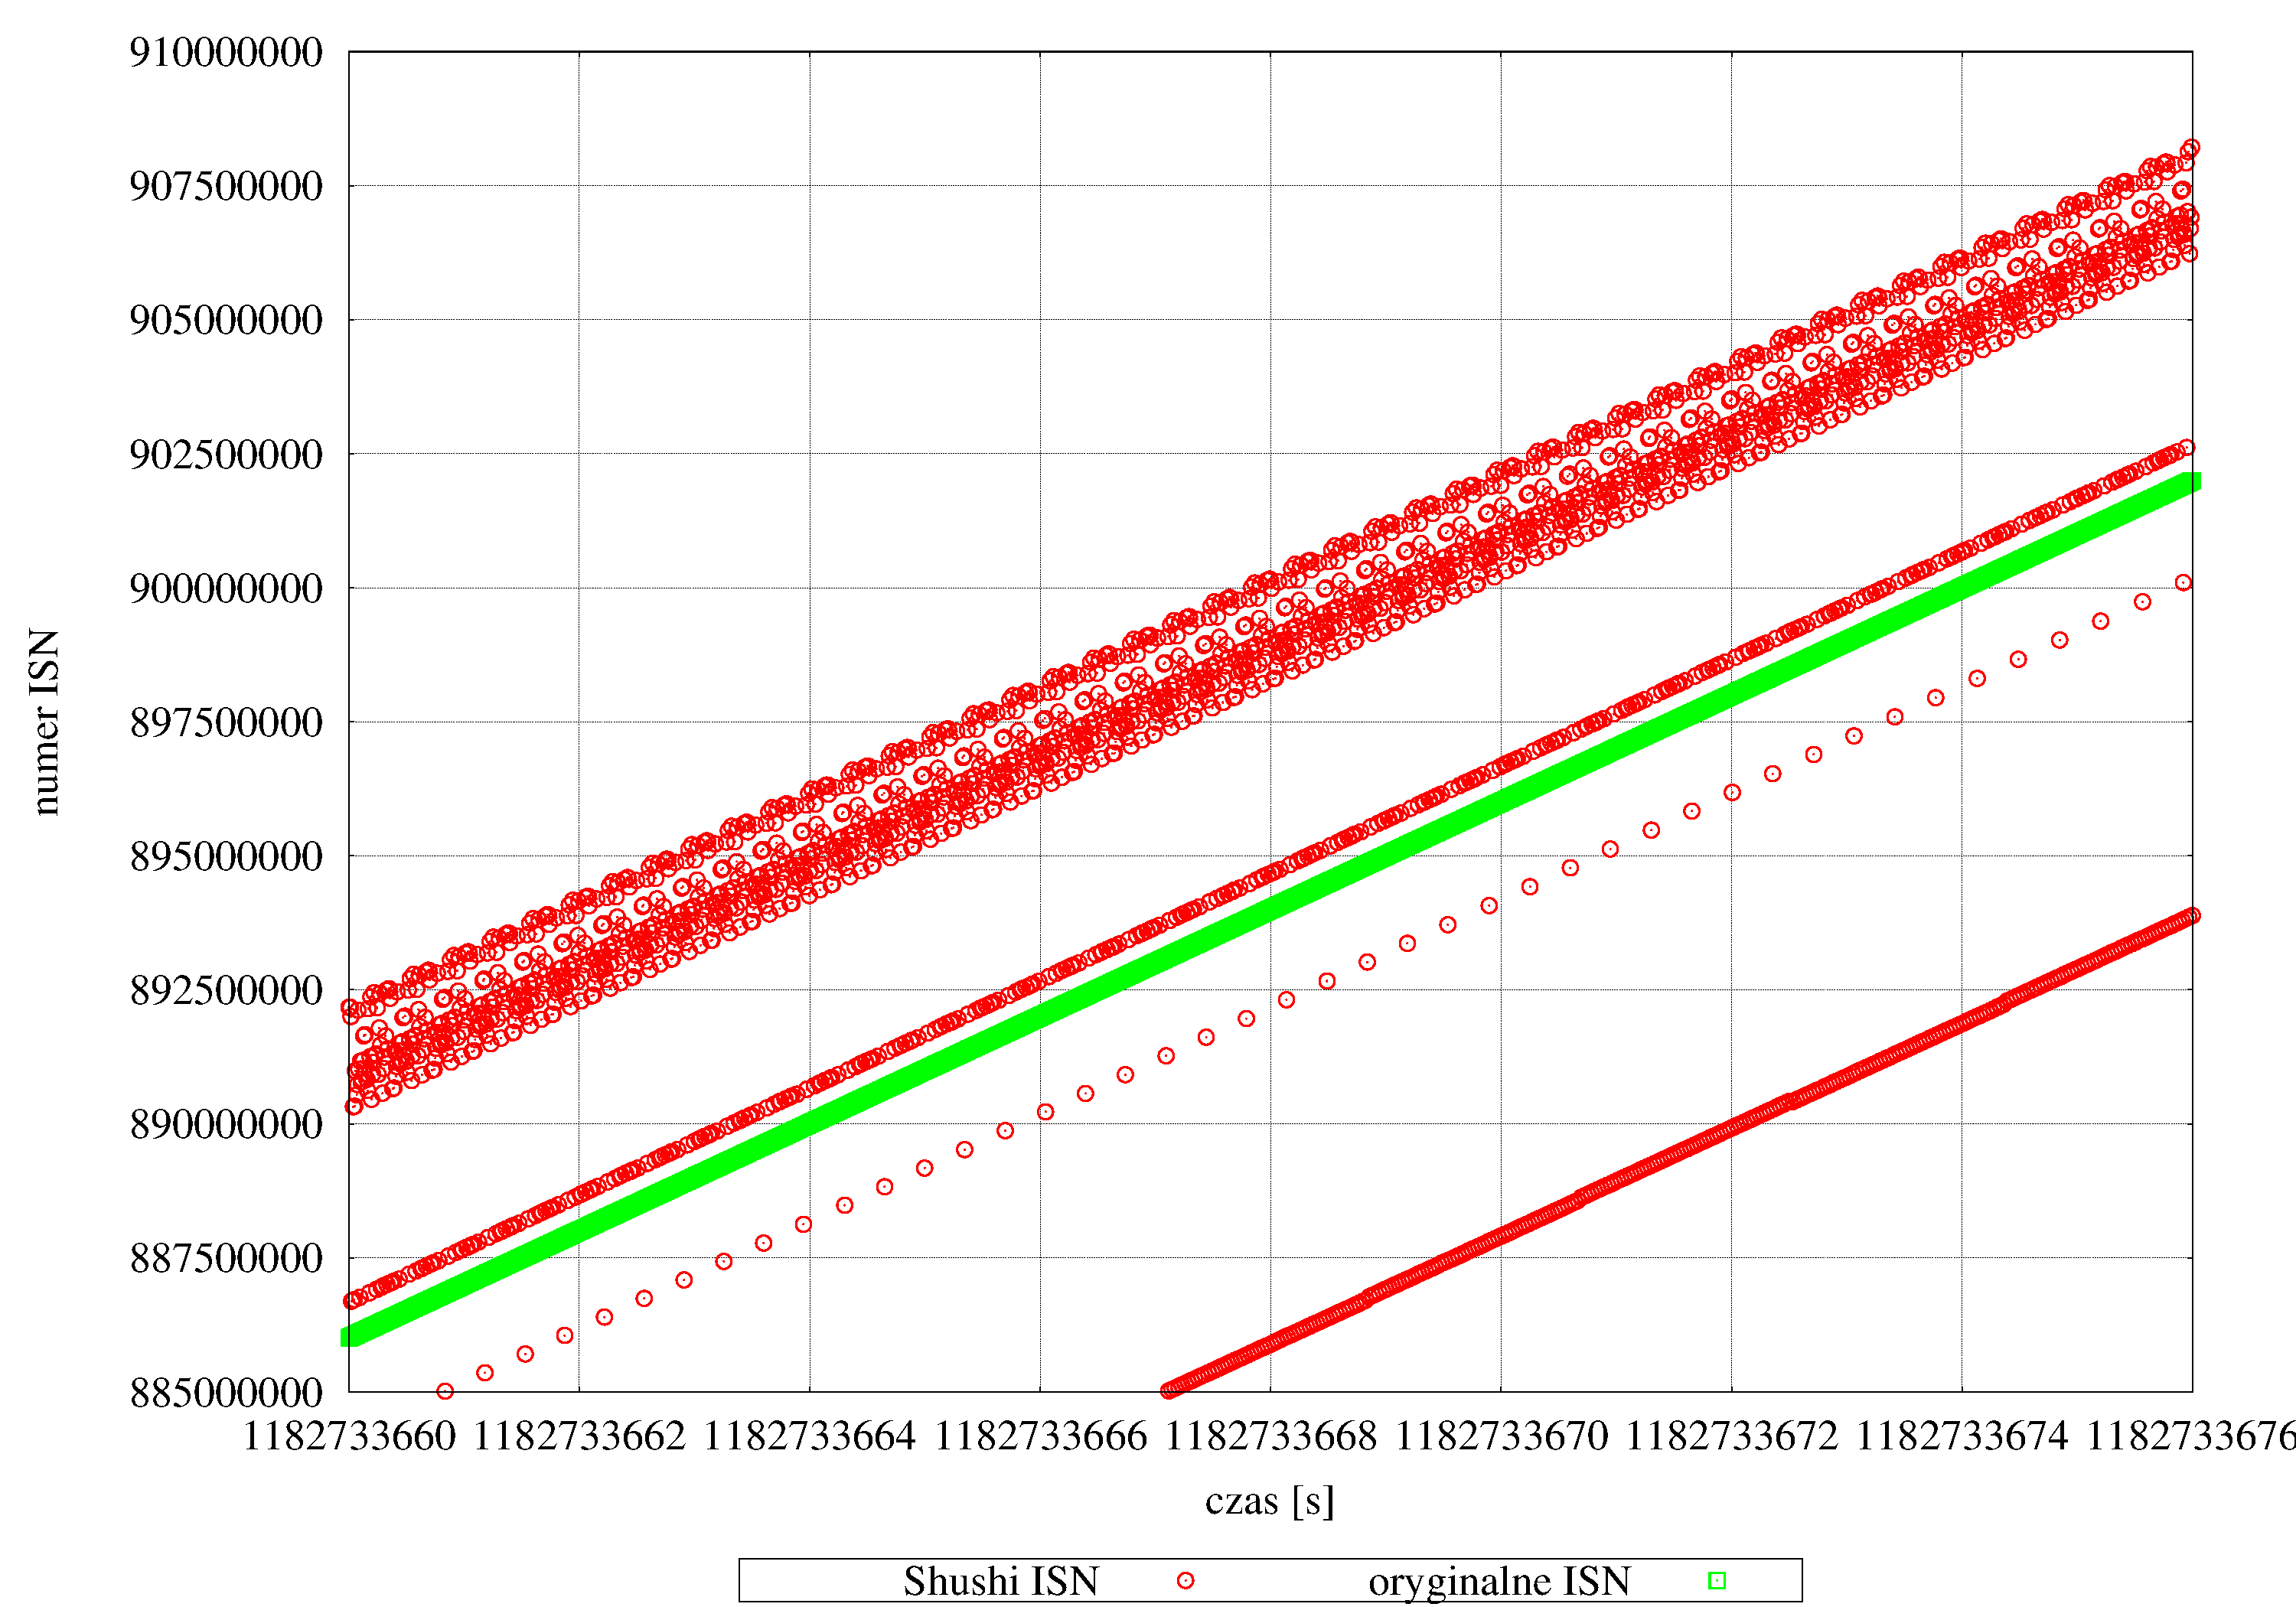
\includegraphics[scale=0.21]{\ImgPath/rys/IPPortConstData.pdf}
\end{center}
	\caption{Numery ISN wygenerowane przez jądro oraz \tech{Shushi}, stałe 
numery IP oraz porty TCP, stałe dane dla \tech{Shushi}, serie po około 2800 
próbek.}
	\label{IPPortConstData}
\end{figure}

\begin{figure}[!htbp]
	\begin{center}
\centering
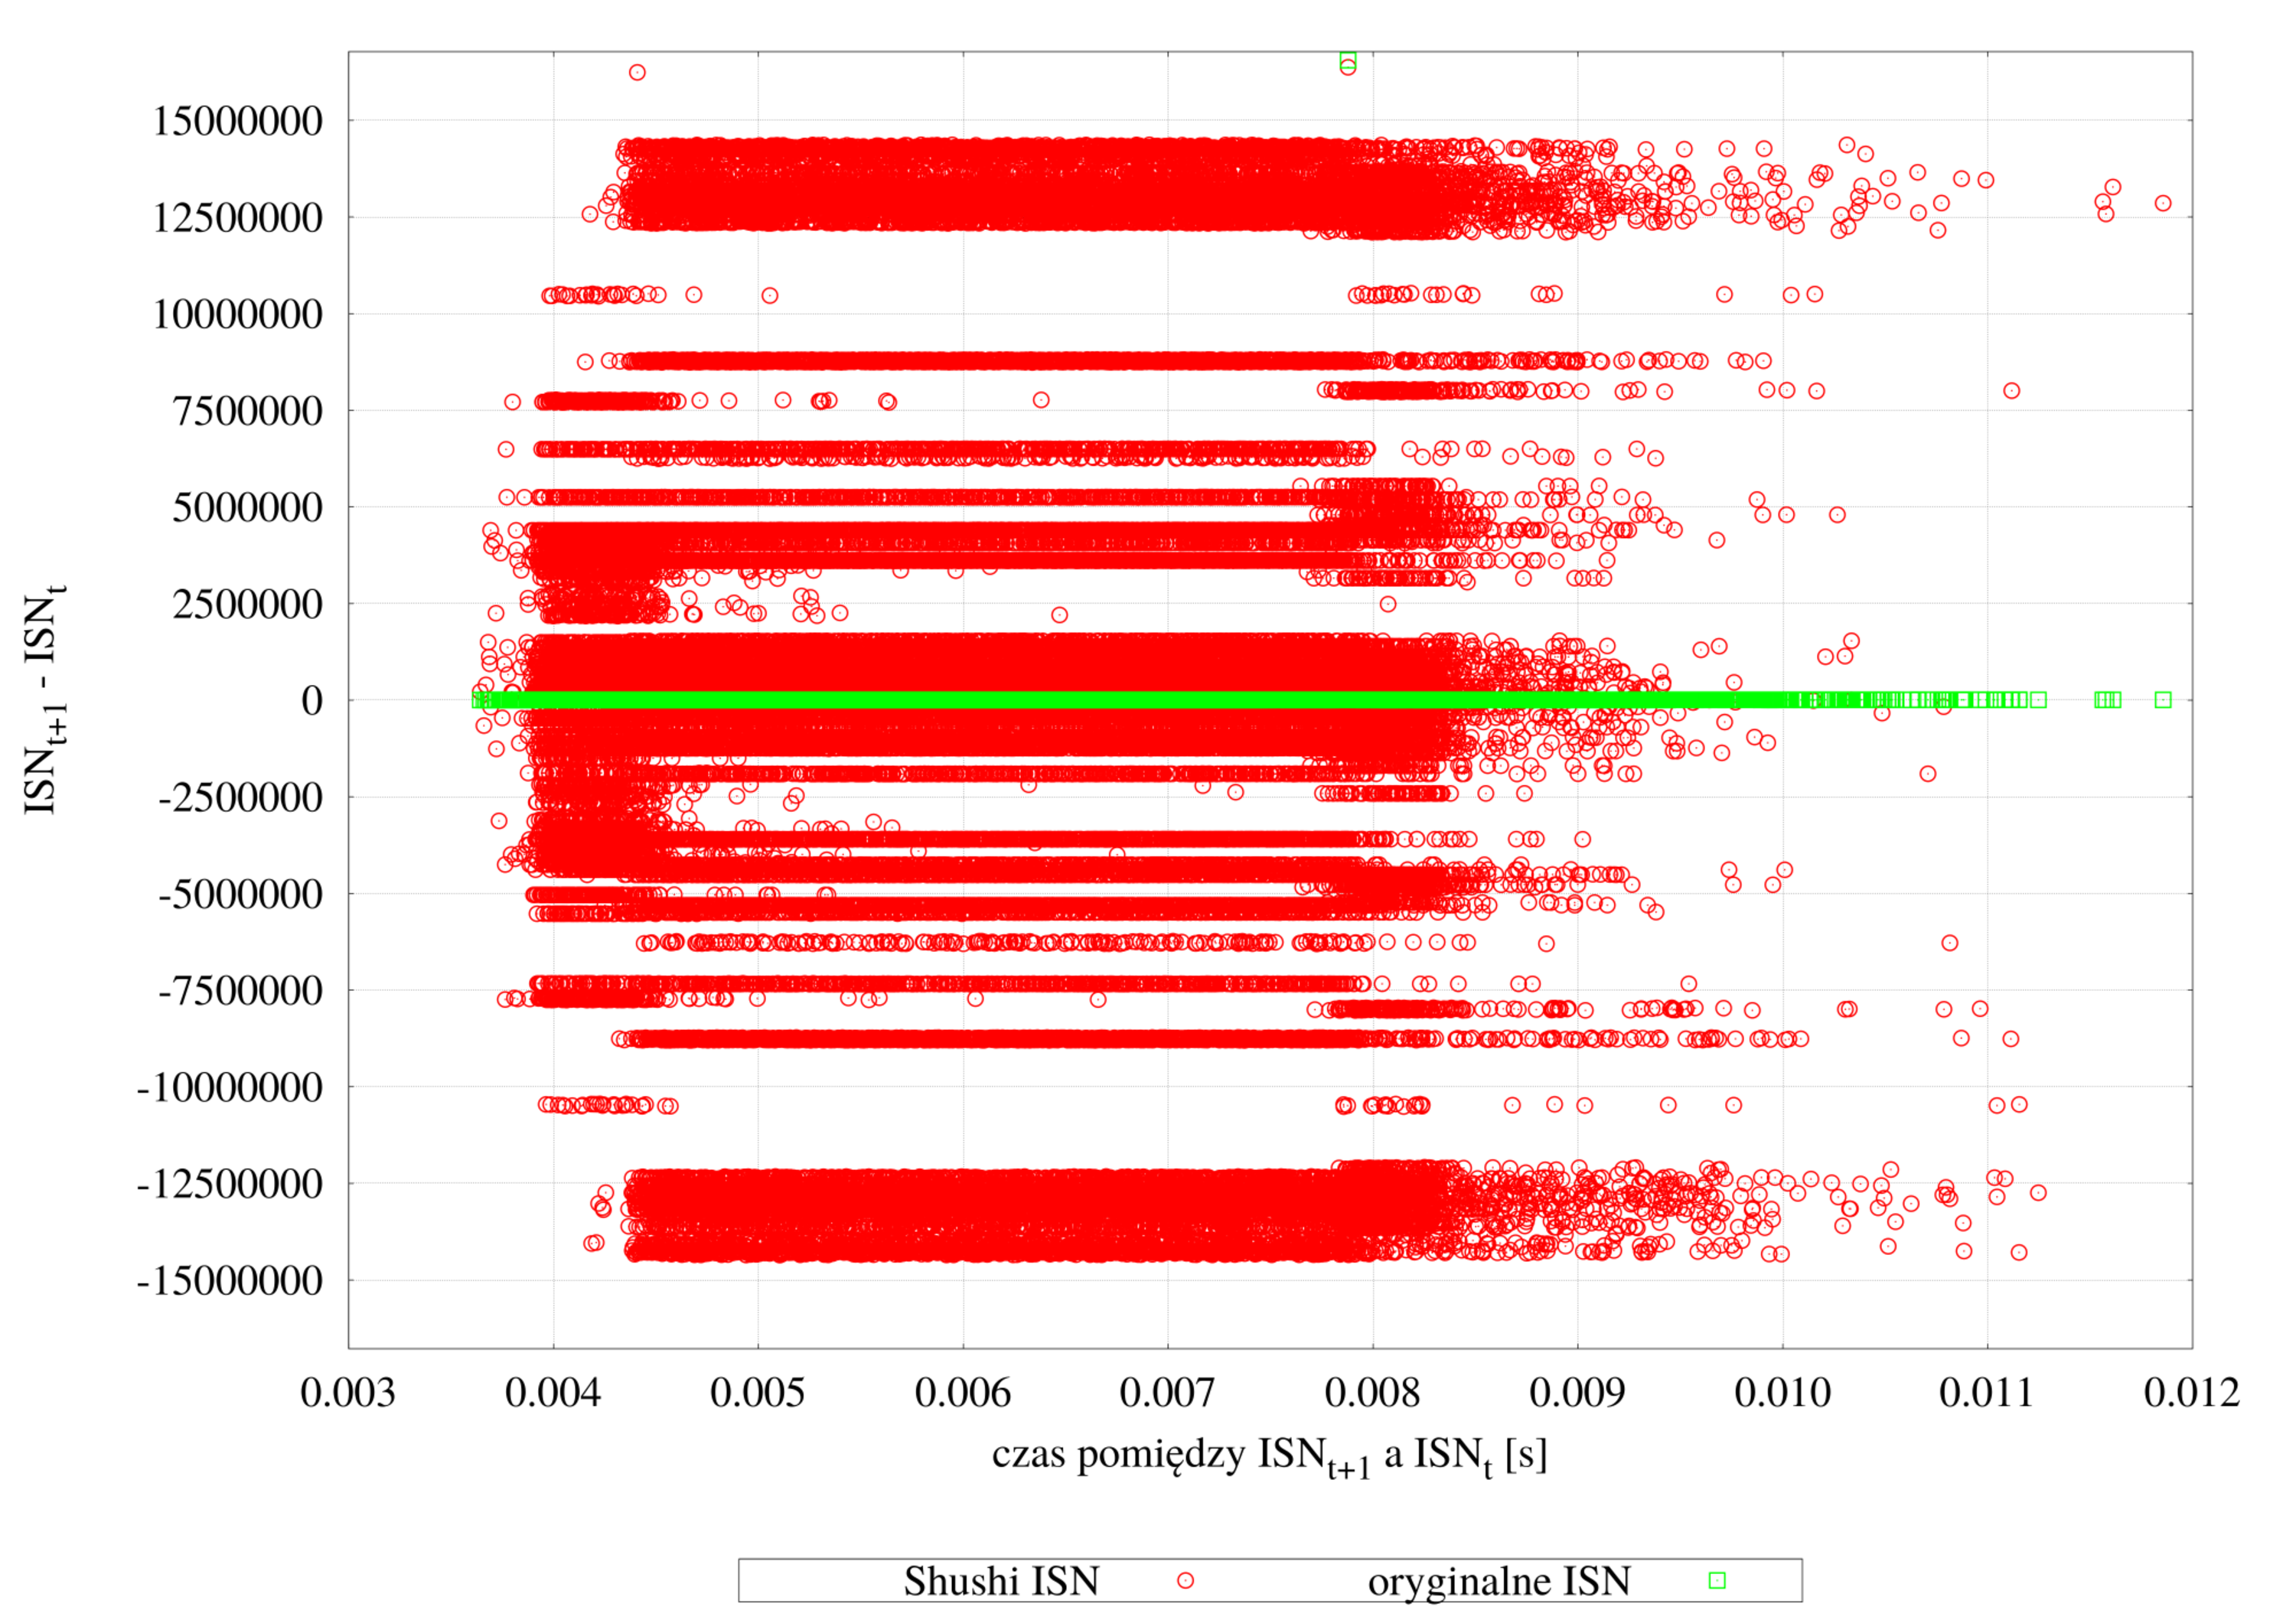
\includegraphics[scale=0.21]{\ImgPath/rys/IPPortConstDataDiff.pdf}
\end{center}
	\caption{Różnice pomiędzy kolejnymi numerami ISN wygenerowanymi przez 
jądro oraz \tech{Shushi}, stałe numery IP oraz porty TCP, stałe dane dla 
\tech{Shushi}, serie po około 60000 próbek.}
	\label{IPPortConstDataDiff}
\end{figure}

\begin{figure}[!htbp]
	\begin{center}
\centering
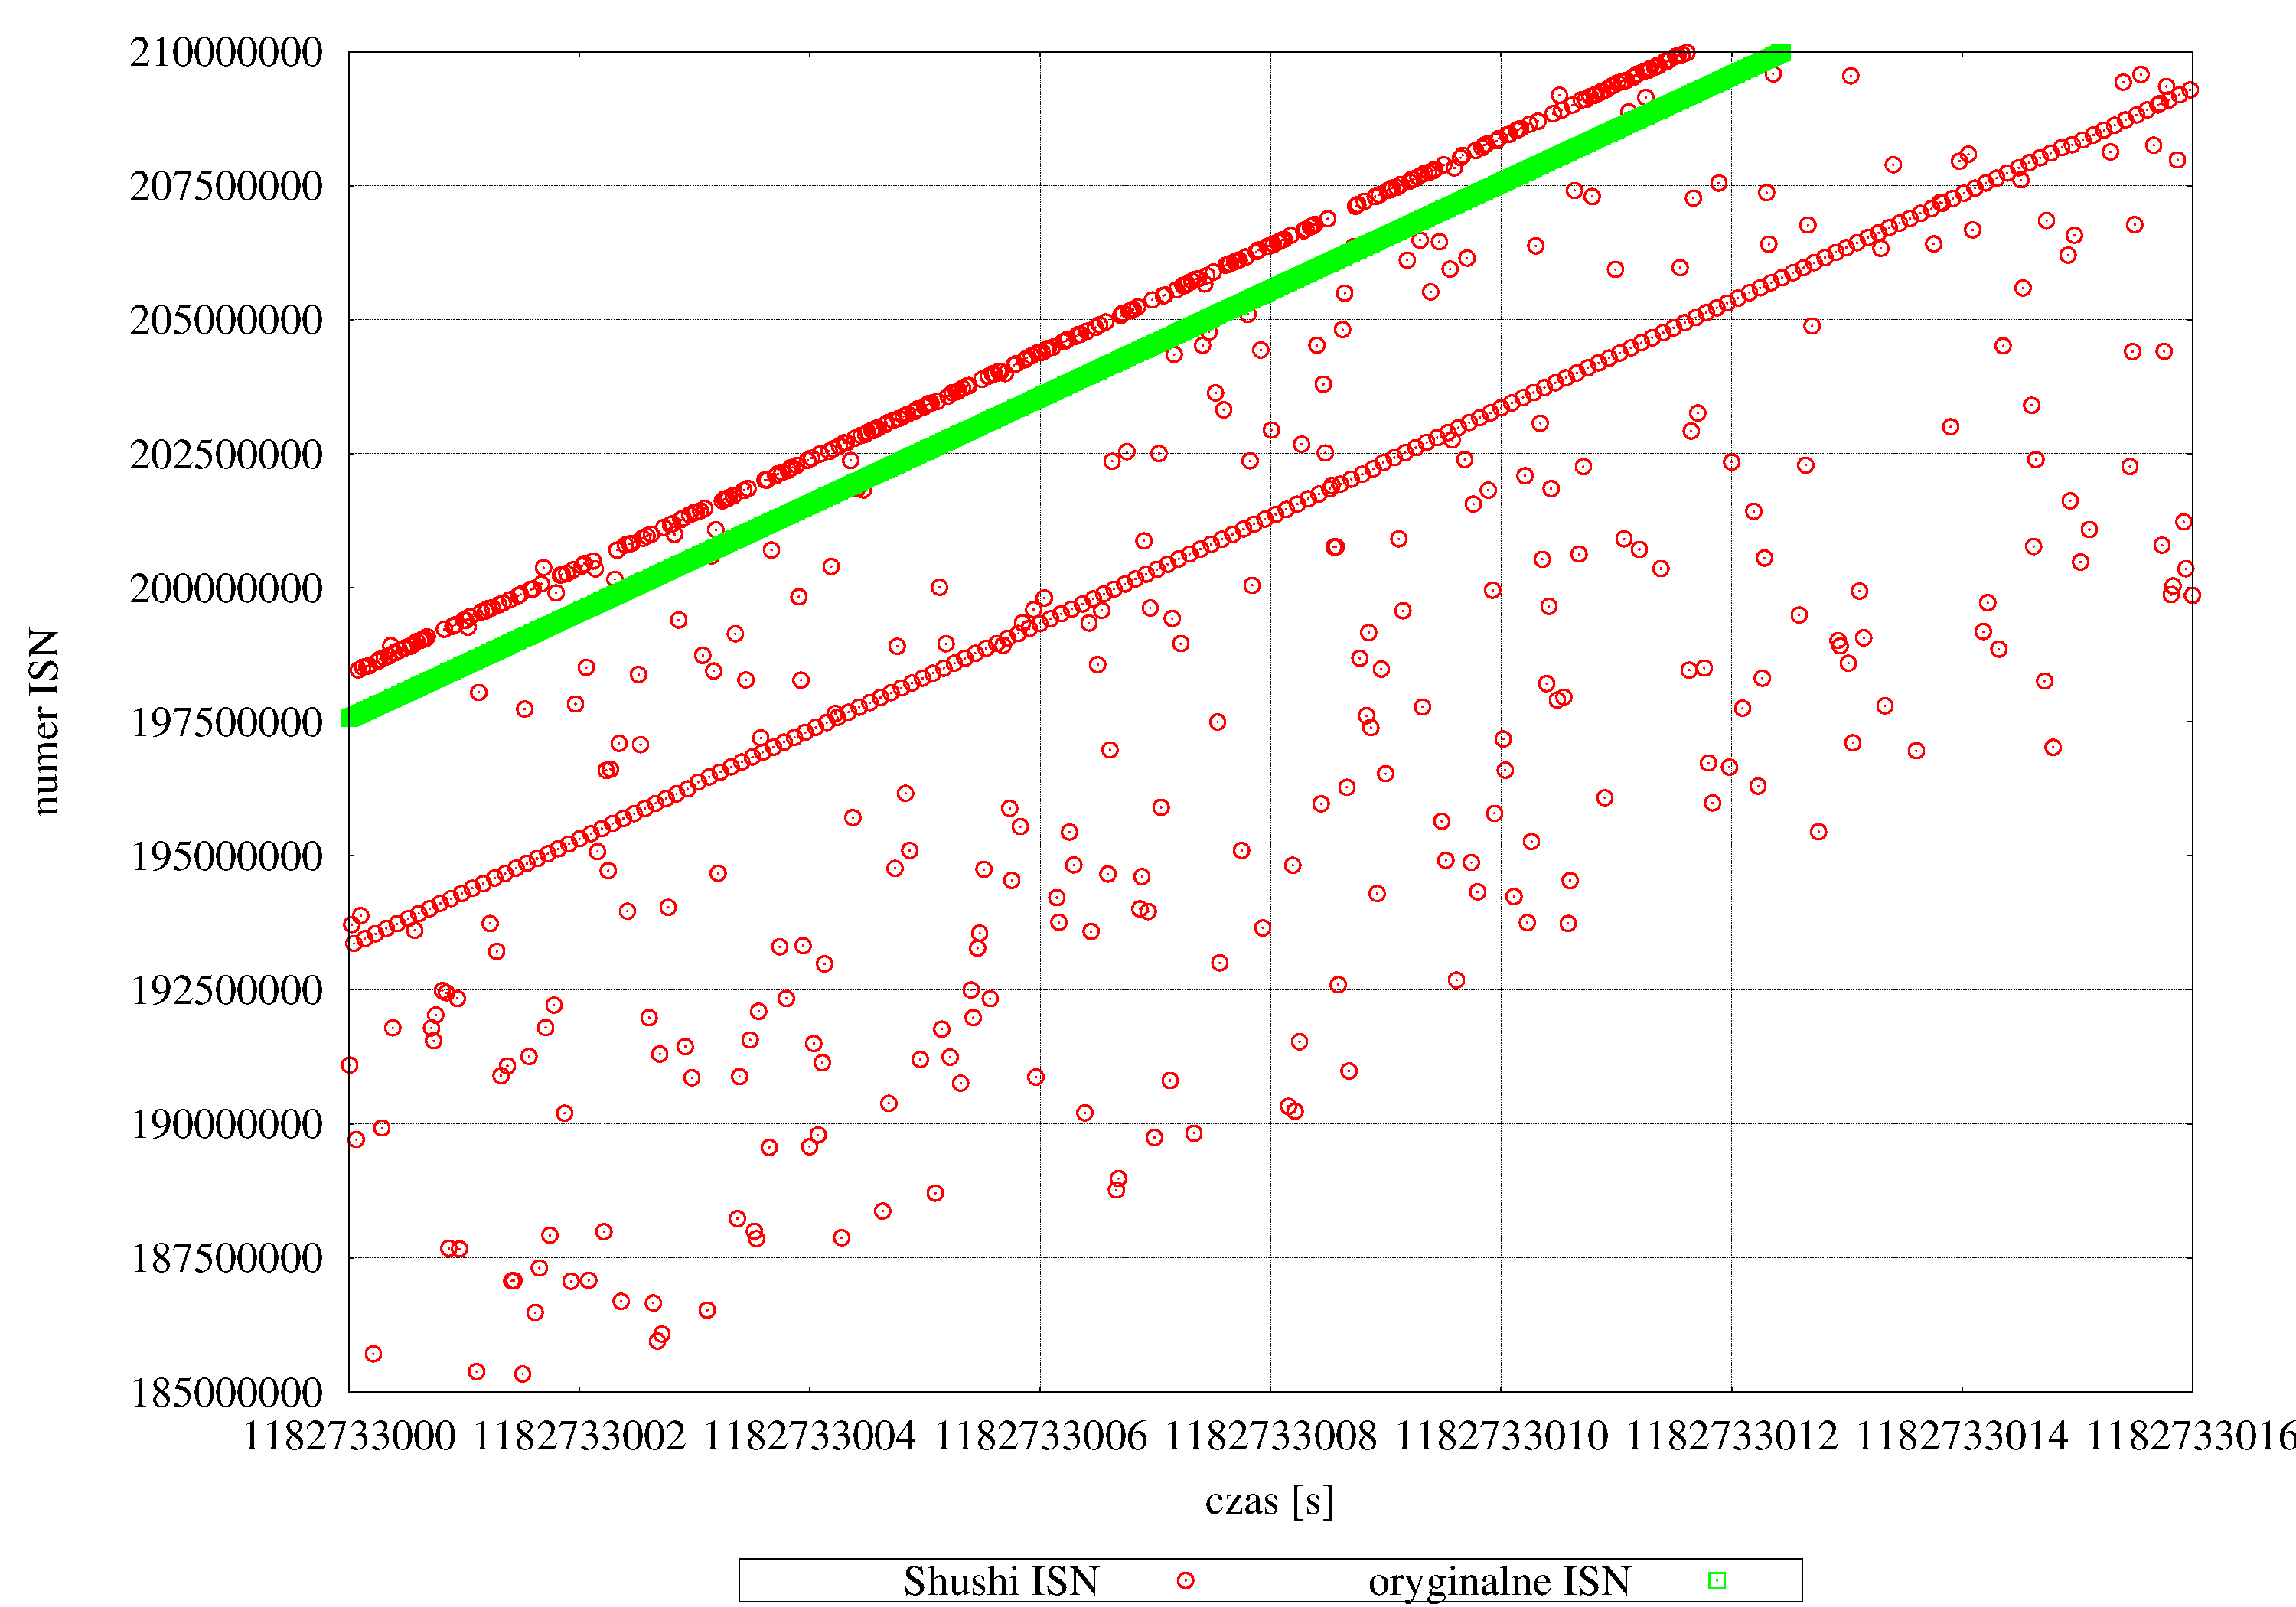
\includegraphics[scale=0.21]{\ImgPath/rys/IPPortRandData.pdf}
\end{center}
	\caption{Numery ISN wygenerowane przez jądro oraz \tech{Shushi}, stałe 
numery IP oraz porty TCP, losowe dane dla \tech{Shushi}, serie po około 860 
próbek.}
	\label{IPPortRandData}
\end{figure}

\begin{figure}[!htbp]
	\begin{center}
\centering
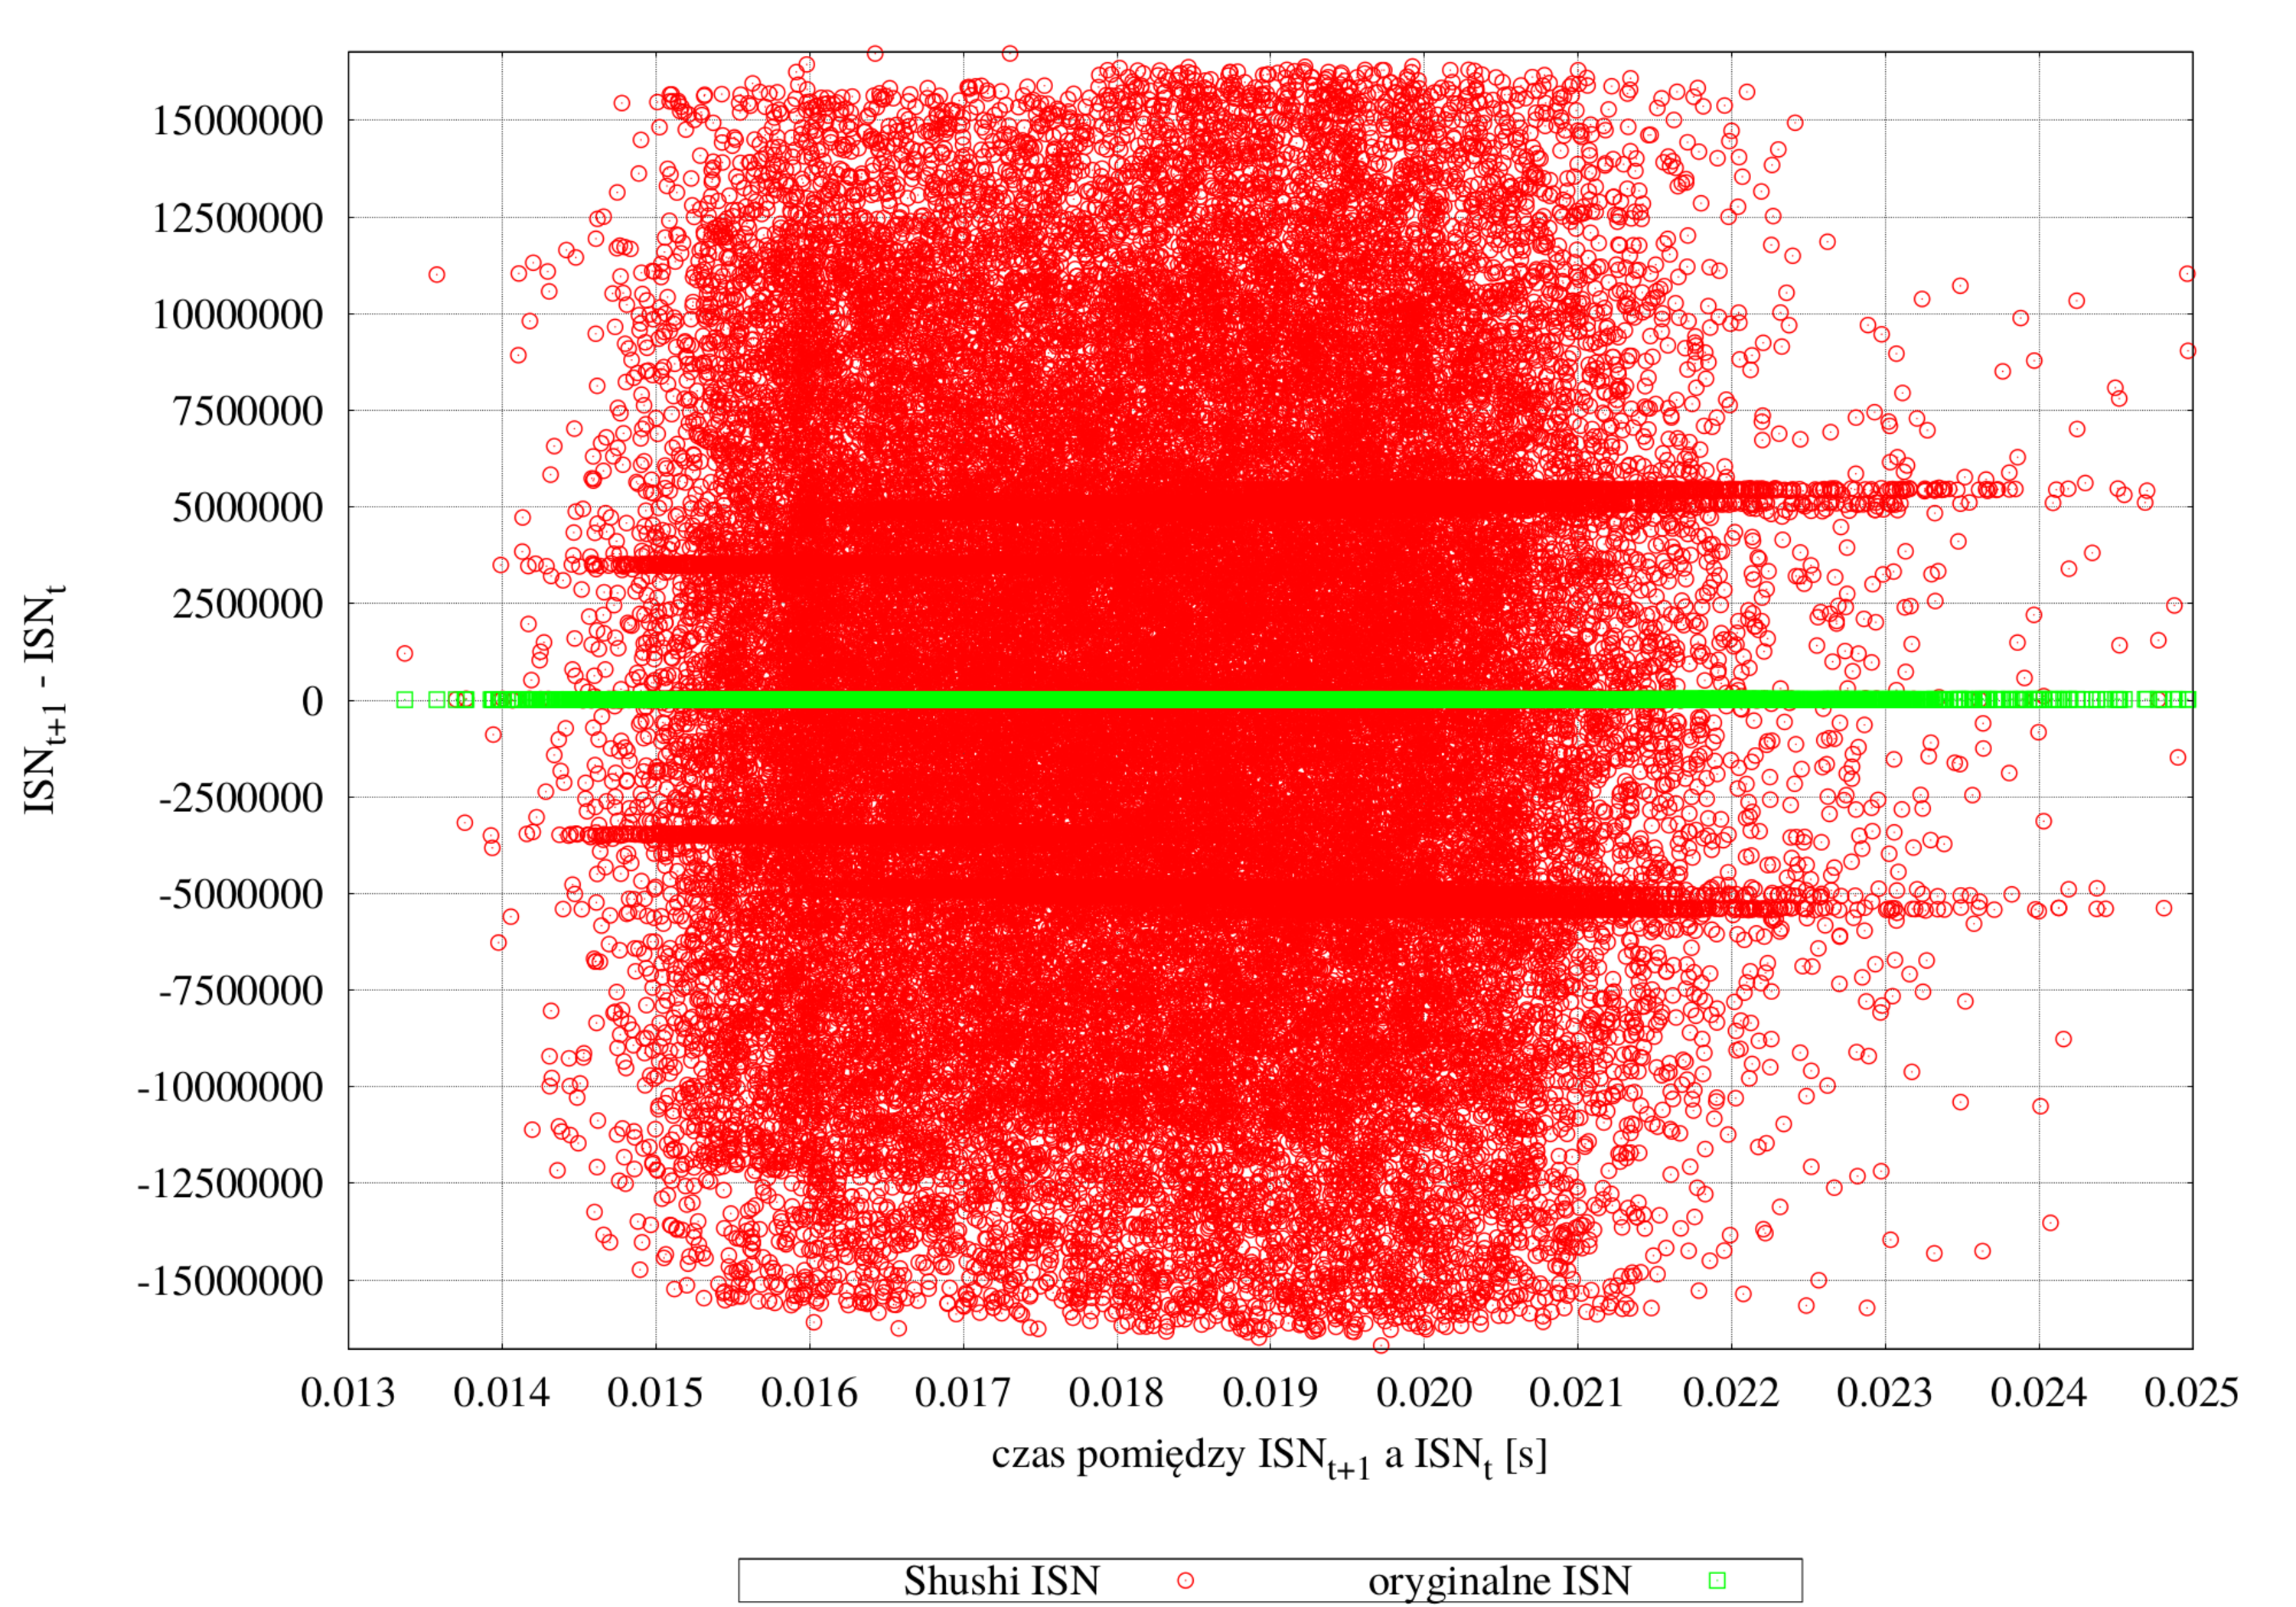
\includegraphics[scale=0.21]{\ImgPath/rys/IPPortRandDataDiff.pdf}
\end{center}
	\caption{Różnice pomiędzy kolejnymi numerami ISN wygenerowanymi przez 
jądro oraz \tech{Shushi}, stałe numery IP oraz porty TCP, losowe dane dla 
\tech{Shushi}, serie po około 60000 próbek.}
	\label{IPPortRandDataDiff}
\end{figure}

\begin{thebibliography}{99}
\addcontentsline{toc}{chapter}{Bibliografia}
\bibitem{who}{ State of Worlds Nursing 2020. Investing in education, job and  leadership; https://apps.who.int/iris/handle/10665/331677. [dostęp 05.02.2022]}
\bibitem{rap}{Najbardziej poważane zawody przez Polaków w 2021; https://swresearch.pl/news/najbardziej-powazane-zawody-przez-polakow-w-2021. [dostęp 05.02.2022]}
\bibitem{zro}{Historia medycyny;https://historiamedycyny.pl/ [dostęp 05.02.2022]}
\bibitem{tlo}{Maksymowicz A. Zagadnienia zawodowe pielęgniarstwa na tle historycznym. Warszawa: Wydawnictwo Lekarskie PZWL; 1977}
\bibitem{flo}{Bostridge M. Florence Nighitingale-The lady with lamp; https://www.bbc.co.uk/history/british/victorians/nightingale-01.shtml [dostęp 05.02.2022]}
\bibitem{linda}{Richards L. Reminescences of Linda Richards. Americas firsttrained nurse.Boston: Whitcomb \& Barrows;2015}
\bibitem{rada}{Poznańska S. Pielęgniarstwo wczoraj i dziś. Warszawa: Wydawnictwo Lekarskie PZWL;1988}
\bibitem{ikon}{Supady J. Początek nowoczesnego pielęgniarstwa w XIX wieku. Health Promotion and Physical Activity. 2019; 2(7)}
\bibitem{ikonpol}{Slosorz T. Kształcenie pielęgniarek w ujęciu historycznym. Polski Przegląd Nauk o Zdrowiu. 2014; 4(41)}
\bibitem{szkol}{Iżycka-Kowalska A. Powstanie Warszawskiej Szkoły Pielęgniarstwa i jej rozwój w latach 1921-1928. Warszawa; Wydawnictwo Lekarskie PZWL; 1989}
\bibitem{50}{Kaniewska-Iżycka J. Rozwój pielęgniarstwa polskiego do 1950 roku. Materiały pomocnicze do historii zawodu pielęgniarskiego cz.1. Centrum Metodyczne Doskonalenia Nauczycieli Średniego Szkolnictwa Medycznego;1987}
\bibitem{czas}{Wolska-Lipiec K. Czasopisma; http://www.wmpp.org.pl/pl/wydawnictwa-pielegniarskie/czasopisma. html. [dostęp 11.02.2022]}
\bibitem{spec}{Hutner R. Kuźnia koncepcji pielęgniarskich.Pielęgniarstwo 2000;1992;3}
\bibitem{model}{Ministerstwo Zdrowia. Nowe kompetencje pielęgniarek i położnych. Warszawa; Fundusze Europejskie. Wiedza Edukacja Rozwój; 2020}
\bibitem{deter}{Sak-Skowron M. Determinanty satysfakcji z pracy. Studium teoretyczne. Marketing i zarządzanie.2017;2(48)}
\bibitem{usta}{Wilczewska L. Rozwój zawodu pielęgniarskiego w ujęciu historycznym. Biuletyn Naczelnej Izby Pielęgniarek i Położnych. Warszawa; 1994}
\bibitem{1935}{Gnich J. Ustawa o zawodzie z 1935 r.; http://www.wmpp.org.pl/pl/ustawa-o-zawodzie.html. [dostęp 11.02.2022]}.
\bibitem{1996}{Ustawa z dnia 5 lipca 1996 r. o zawodach pielęgniarki i położnej.; https://isap.sejm.gov.pl/isap.nsf/DocDetails.xsp?id=WDU19960910410 [dostęp 11.02.2022]}
\bibitem{2011}{Ustawa z dnia 15 lipca 2011 r. o zawodach pielęgniarki i położnej.; https://isap.sejm.gov.pl/isap.nsf/DocDetails.xsp?id=wdu20111741039 [dostęp 11.02.2022]}
\bibitem{nipip}{Ustawa z dnia 1 lipca 2011 r. o samorządzie pielęgniarek i położnych.; http://isap.sejm.gov.pl/isap.nsf/DocDetails.xsp?id=WDU20111741038 [dostęp 11.02.2022]}
\bibitem{prawo}{Karkowska D. Prawo medyczne dla pielęgniarek. Warszawa: Wolters Kluwer; 2020}
\bibitem{akty}{Akty prawne w dziedzinie pielęgniarstwa.; https://isap.sejm.gov.pl/isap.nsf/ByKeyword.xsp?key=pielęgniarstwo [dostęp 11.02.2022]}
\bibitem{strategia}{ Ministerstwo Zdrowia. Polityka wieloletnia państwa na rzecz pielęgniarstwa i położnictwa w Polsce. Warszawa; Fundusze Europejskie.Wiedza Edukacja Rozwój ; 2020}
\bibitem{federic}{ Laloux F. Pracować inaczej. Nowatorski model organizacji inspirowany kolejnym etapem rozwoju ludzkiej świadomości. Warszawa; Studio Emka; 2015}
\bibitem{ile}{Strzelec P. Nowe uprawnienia, nowe roszczenia-aspekty odpowiedzialności prawnej pielęgniarek i położnych. Bydgoszcz; Okręgowa Izba Pielęgniarek i Położnych; 2018}
\bibitem{strajk}{Związek i jego historia. Ogólnopolski Związek Zawodowy Pielęgniarek i Położnych; https://ozzpip.pl/about/ [dostęp 11.02.2022]}.
\bibitem{julia}{Osiecka J. Powrót do młodych lat; https://www.queensilvianursingaward.com/pl-stories/powrot-do-mlodych-lat [dostęp 11.02.2022]}.
\bibitem{dorota}{ Kilańska D. Nowe role i zadania pielęgniarki w XXI w. Gabinet Prywatny; 2012: 7/8}
\bibitem{petycja}{Petycja. Rozszerzenie kompetencji pielęgniarek i położnych. https://www.rynekzdrowia.pl/Polityka-zdrowotna/Pielegniarki-chca-szerszych-kompetencji-Wystawiania-L4-recept-i-skierowan-na-szczepienia,229508,14.html [dostęp 20.02.2022]}
\bibitem{poz}{Pielęgniarki w zespole do spraw POZ. https://www.rynekzdrowia.pl/Polityka-zdrowotna/Pielegniarki-chca-pracowac-nad-zmianami-w-POZ-Chca-dolaczyc-do-zespolu-powolanego-przez-ministra,229668,14.html [dostęp 20.02.2022]}
\bibitem{badania}{Felsmann M, Głowacka M, Haor B, Humańska M, Kurowska K, Rezmerska L, et al. Badania fizykalne jako integralny element pracy pielęgniarki. Bydgoszcz; 2006}
\bibitem{spoty}{Latos M. Krew i mózg; https://open.spotify.com/show/643Y5GdI7yGkqVxzPaBvSH [dostęp 16.02.2022]}
\bibitem{zdrowie}{Andruszkiewicz A. Nowik M Zachowania zdrowotne kobiet czynnych zawodowo. Problemy Pielęgniarstwa. 2011; (19)}

%książka
\bibitem{obciążenia}{Ksykiewicz-Dorota A. Podstawy organizacji pracy pielęgniarskiej. Lublin; Czelej; 2004}

\bibitem{statystyka}{Raport NIPIP: Katastrofa kadrowa pielęgniarek i położnych. Warszawa; NIPIP; 2021 [dostęp 16.02.2022]}
\bibitem{zgony}{Ile żyje polska pielęgniarka. Wyjaśniamy  wątpliwości wokół danych NIPIP; https://demagog.org.pl/analizy i raporty/ile-zyje-polska-pielegniarka-wyjasniamy-watpliwosci-wokol-danych-nipip/ [dostęp 18.02.2022]}.
\bibitem{sen}{Current psychiatry report. Medical College of Georgia at Augusta University. Frontiers Ottawa. 2021; https://www.mp.pl/covid19/covid19-aktualnosci/270418,pandemiczna-bezsennosc-medykow [dostęp 18.02.2022]}
\bibitem{covid}{Biegańska-Banaś J. Makara-Studzińska. Strategie radzenia sobie pielęgniarek podczas pandemii Covid-19. Problemy Pielęgniarstwa 2020/1}
\bibitem{cyfrowe}{Lewoniewska J. Zarobki i dodatkowe zatrudnienie pielęgniarek i położnych w Polsce. Raport Stowarzyszenia Pielęgniarki Cyfrowe; 2021;https://www.pielegniarkicyfrowe.pl/2021/06/12/zarobki-i-dodatkowe-zatrudnienie-pielegniarek-i-poloznych-w-polsce/[dostęp 18.02.2022]}
\bibitem{stanowisko}{Bujanowska M. Żółtańska J. Zawodowe zagrożenia zdrowia pracowników ochrony zdrowia w miejscu pracy. Zeszyty Naukowe PWSZ. Legnica; 2010;(6)}
\bibitem{skutki}{Zużlewicz K. Skutki zdrowotne pracy w systemie w niefizjologicznym rytmie. Zeszyty Naukowe SGSP. 2017; nr 62 (1/2)}
\bibitem{p.p}{Bilski B. Wpływ pracy zmianowej na sposób odżywiania się i patologię przewodu pokarmowego wśród pielęgniarek. Medycyna Pracy. Wyniki badania pilotażowego. 2006; 57 (1)}
\bibitem{wykaz}{Rozporządzenie Rady Ministrów  w sprawie chorób zawodowych z 2009 r. DZ.U.2013.1367. https://sip.lex.pl/akty-prawne/dzu-dziennik-ustaw/choroby-zawodowe-17551901 [dostęp 18.02.2022]}
\bibitem{skuteczność}{Gromulska L. Cianciara D. Piotrowicz M. Własna skuteczność w modelach zachowań zdrowotnych oraz w edukacji zdrowotnej. Przegląd epidemiologiczny. 2009; (63)}.
\bibitem{salutogeneza}{Heszen-Celińska I. Sęk H. Psychologia zdrowia. Warszawa; Wydawnictwo Naukowe PWN; 2021}
\bibitem{stres}{Bartkowiak G. Człowiek w pracy. Od stresu do sukcesu w organizacji. Warszawa; Wydawnictwo Ekonomiczne; 2009}
\bibitem{hipoteza}{Tomaszewska-Lipiec R. Relacje praca-życie pozazawodowe. Bydgoszcz; Wydawnictwo Uniwersytetu Kazimierza Wielkiego; 2014}
\bibitem{relacja}{Lachowska B. Wzajemne oddziaływanie pracy i rodziny-perspektywa konfliktu i falicytacji. Raport z badań pilotażowych. Łódź; Wydawnictwo Uniwersytetu Łódzkiego; 2008}
\bibitem{konflikt}{Siemiginowska P. Iskra-Golec I. Wątroba J. Relacja praca/rodzina, zadowolenie z pracy i życia oraz zdrowie u pielęgniarek zmianowych i dziennych. Studia Psychologica. 2014; VII}
\bibitem{dzieci}{ Frączyk J.  Pierwsze dziecko po trzydziestce. https://businessinsider.com.pl/finanse/makroekonomia/wiek-kobiet-przy-porodzie-pierwszego-dziecka-ciagle-rosnie-co-z-systemem-emerytalnym/c801ke5 [dostęp 18.02.2022]}
\bibitem{urlop}{ Podrażka M. Urlop macierzyński. https://www.gov.pl/web/rodzina/urlop-macierzynski [dostęp 18.02.2022]}
\bibitem{wywiad}{Kapusta P. Pandemia. Raport z linii frontu. Lubicz; Wydawnictwo Insignis; 2020}
\bibitem{rozwody}{ Lekarze rozwodzą się rzadziej niż prawnicy. https://pulsmedycyny.pl/lekarze-rozwodza-sie-rzadziej-niz-prawnicy-875944 [dostęp 18.02.2022]}
\bibitem{melibruda}{Melibruda J. Ja - Ty - My. Warszawa; Instytut Psychologii Zdrowia PTP; 2003}
\bibitem{wzbogacanie}{Greenhaus J.H. Powell G.N. When work and family are alies; A theory of work-lfamily enrichment. Acadamy of Management Review. 2006 (vol 31/1)}
\bibitem{bezpieczeństwo}{Jabłońska A. Bezpieczeństwo pracy w Polsce 2019. Mobbing, depresja, stres w miejscu pracy. Koalicja Bezpieczni w pracy. 2019; http://bezpieczniwpracy.pl/wp-content/uploads/2019/10/Raport-Bezpieczeństwo-Pracy-w-Polsce-2019.pdf [dostęp 18.02.2022]}
\bibitem{prężność}{ Falewicz A. Prężność osobowości i jej rola w procesach radzenia sobie ze stresem. Studia Koszalińsko-Kołobrzeskie. 2016; 23} 
\bibitem{talent}{https://pielegniarskiswiat.pl/ [dostęp 18.02.2022]}
\bibitem{sport}{Chuchra M. Gorbaniuk J. Aktywność fizyczna pielęgniarek. Badania porównawcze. Pielęgniarstwo Polskie 2017 2(64)}
\bibitem{izby}{https://www.doipip.wroc.pl/dla-pielegniarki-i-poloznej/ [dostęp 18.02.2022]}
\bibitem{jak}{ Rubinkowska A. Jak wesprzeć zdrowie psychiczne pracowników medycznych. Warszawa;  Wiedza i Praktyka; 2021}
\bibitem{projekt}{https://medstres.sos.pl/ [dostęp 18.02.2022]}
\bibitem{anita}{https://www.profinfo.pl/autorzy/anita-galeska-sliwka,9090.html [dostęp 18.02.2022]}

\bibitem{krys}{Lutyńska K. Wywiad kwestionariuszowy. Kraków; Wydawnictwo PAN; 1984}

\bibitem{mich}{Łobocki M. Wprowadzenie do metodologii badań pedagogicznych. Kraków; Wydawnictwo Impuls; 1999}

\bibitem{janusz}{Sztumski J. Wstęp do metod i technik badań społecznych. Katowice; Wydawnictwo Śląsk; 1999}

\bibitem{tadeusz}{Pilch T. Metodologia pedagogicznych badań środowiskowych. Warszawa; Państwowe Wydawnictwo Naukowe, 1980}

\bibitem{winc}{Okoń W. Nowy słownik pedagogiczny. Warszawa; Wydawnictwo Znak; 1999}

\end{thebibliography}

\zakonczenie  % wklejenie recenzji i opinii

\end{document}
%+++ END +++
